\documentclass[11pt,a4paper]{article}

% --- Core Packages ---
\usepackage[utf8]{inputenc}
\usepackage[margin=2.2cm,top=2.5cm,bottom=2.5cm]{geometry}
\usepackage{amsmath,amsfonts,amssymb}
\usepackage{graphicx}
\usepackage{booktabs}
\usepackage{array}
\usepackage{listings}
\usepackage{xcolor}
\usepackage{tikz}
\usetikzlibrary{arrows.meta,positioning,shapes.geometric,fit,calc}
\usepackage{hyperref}
\usepackage{fancyhdr}
\usepackage{caption}
\usepackage{float}

% --- Hyperlink Settings ---
\hypersetup{
    colorlinks=true,
    linkcolor=blue!70!black,
    citecolor=green!60!black,
    urlcolor=blue!80!black
}

% --- Headers and Footers ---
\pagestyle{fancy}
\fancyhf{}
\fancyhead[L]{\small \textbf{Analysis of Algorithms} -- Lab 09: Greedy Technique}
\fancyhead[R]{\small \textbf{Yachay Tech University}}
\fancyfoot[C]{\thepage}
\renewcommand{\headrulewidth}{0.6pt}
\renewcommand{\footrulewidth}{0.4pt}

% --- Listings Settings for C / C++ ---
\definecolor{codegreen}{rgb}{0,0.6,0}
\definecolor{codegray}{rgb}{0.5,0.5,0.5}
\definecolor{codepurple}{rgb}{0.58,0,0.82}
\definecolor{backcolour}{rgb}{0.97,0.97,0.98}
\definecolor{terminalbg}{rgb}{0.12,0.12,0.14}
\definecolor{terminalfg}{rgb}{0.9,0.9,0.9}

\lstdefinestyle{cstyle}{
    backgroundcolor=\color{backcolour},   
    commentstyle=\color{codegreen},
    keywordstyle=\color{blue}\bfseries,
    numberstyle=\tiny\color{codegray},
    stringstyle=\color{codepurple},
    basicstyle=\ttfamily\footnotesize,
    breakatwhitespace=false,         
    breaklines=true,                 
    captionpos=b,                    
    keepspaces=true,                 
    numbers=left,                    
    numbersep=6pt,                  
    showspaces=false,                
    showstringspaces=false,
    showtabs=false,                  
    tabsize=2,
    frame=single,
    rulecolor=\color{gray!40}
}

\lstdefinestyle{terminalstyle}{
    backgroundcolor=\color{terminalbg},
    basicstyle=\ttfamily\footnotesize\color{terminalfg},
    breaklines=true,
    frame=single,
    rulecolor=\color{gray!60},
    numbers=none
}

% --- TikZ Styles for Graphs ---
\tikzset{
    vertex/.style = {circle, draw=black, fill=white, inner sep=0pt, minimum size=24pt, font=\bfseries},
    mstvertex/.style = {circle, draw=blue!80!black, fill=blue!10, inner sep=0pt, minimum size=24pt, font=\bfseries},
    edge/.style = {thick},
    diredge/.style = {thick, -{Latex[length=3mm, width=2mm]}},
    mstedge/.style = {ultra thick, draw=blue!70!black},
    weight/.style = {fill=white, inner sep=1.5pt, font=\footnotesize\bfseries}
}

% --- Title and Metadata ---
\title{
    \vspace{-1.4cm}
    \begin{minipage}{0.48\textwidth}
        \flushleft
        
\includegraphics[height=1.3cm]{fotos/logo1.png}
    \end{minipage}%
    \hfill
    \begin{minipage}{0.48\textwidth}
        \flushright
        
\includegraphics[height=1.3cm]{fotos/logo2.png}
    \end{minipage}\\[0.5cm]
    \Large \textbf{UNIVERSIDAD DE INVESTIGACIÓN DE TECNOLOGÍA EXPERIMENTAL YACHAY TECH}\\[0.15cm]
    \large \textbf{School of Mathematical and Computational Sciences}\\[0.25cm]
    \Large \textbf{Course: Analysis of Algorithms (AoA)}\\[0.2cm]
    \LARGE \textbf{Laboratory Report 09: Greedy Technique}\\[0.25cm]
    \large \textit{Prim's Algorithm, Dijkstra's Algorithm, and Huffman Coding}
}
\author{
    \textbf{Author:} Student Laboratory Report \\
    \textbf{Course:} Analysis of Algorithms \\
    \textbf{Institution:} Yachay Tech University
}
\date{\today}

\begin{document}

\maketitle
\thispagestyle{empty}

\begin{abstract}
This report presents an exhaustive theoretical and practical analysis of \textbf{Laboratory 09: Greedy Technique} for the Analysis of Algorithms course at Yachay Tech University. The practice investigates three foundational problems in combinatorial optimization: (1) Minimum Spanning Tree (MST) construction using Prim's algorithm on a weighted undirected graph with full priority queue tracing; (2) design and implementation of Prim's algorithm in standard C and modern C++; (3) analytical step-by-step resolution of the Single-Source Shortest-Paths (SSSP) problem via Dijkstra's algorithm across two distinct instances (a 5-vertex directed graph and a 12-vertex interconnected network); (4) computational implementation of Dijkstra's algorithm in C and C++; and (5) analysis, binary tree synthesis, string encoding, and sequence decoding using optimal Huffman Coding. All software implementations were compiled under the C11 and C++17 standards with strict optimization and warning flags, confirming exact agreement with analytical derivations.
\end{abstract}

\vspace{0.4cm}
\hrule
\vspace{0.6cm}

% ==============================================================================
\section{Introduction and Theoretical Framework}
% ==============================================================================

The \textbf{Greedy Technique} is a foundational algorithmic design paradigm applied to solve optimization problems. Unlike global strategies such as dynamic programming or brute-force search, a greedy algorithm makes the locally optimal choice at each sequential step with the expectation that these immediate decisions will lead to a globally optimal solution.

\subsection{Conditions for Greedy Optimality}
A greedy strategy is guaranteed to find a global optimum if and only if the underlying problem exhibits two primary characteristics:
\begin{enumerate}
    \item \textbf{Greedy Choice Property:} A globally optimal solution can be assembled incrementally by making locally optimal (greedy) choices without reconsidering earlier choices (no backtracking).
    \item \textbf{Optimal Substructure:} An optimal solution to the global problem incorporates optimal solutions to its constituent subproblems.
\end{enumerate}

\subsection{Prim's Algorithm for Minimum Spanning Trees (MST)}
Given a connected, weighted, undirected graph $G = (V, E, w)$, a Minimum Spanning Tree is an acyclic subgraph $T = (V, E_T)$ spanning all vertices $V$ while minimizing the aggregate edge weight:
\begin{equation}
    W(T) = \sum_{e \in E_T} w(e)
\end{equation}
Prim's algorithm initializes the tree with an arbitrary root vertex $v_0$ ($V_T = \{v_0\}$) and iteratively extends $V_T$ by selecting the vertex $u \in V \setminus V_T$ that minimizes the connection cost to any vertex currently in $V_T$. The remaining vertices $V \setminus V_T$ are organized in a priority queue where each vertex is tracked by its label $u(\text{parent}, \text{key})$.

\subsection{Dijkstra's Algorithm for Single-Source Shortest Paths (SSSP)}
Given a directed or undirected graph $G = (V, E, w)$ with non-negative edge weights ($w(e) \ge 0$), Dijkstra's algorithm computes the shortest-path distance from a specified source vertex $s \in V$ to every other vertex in $V$. The algorithm maintains a set of resolved vertices $V_T$. At each step, it extracts the unresolved vertex $u^* \in V \setminus V_T$ possessing the minimum tentative distance $d(u^*)$, adds it to $V_T$, and relaxes each outgoing neighbor:
\begin{equation}
    d(v) \leftarrow \min \left( d(v), \; d(u^*) + w(u^*, v) \right)
\end{equation}

\subsection{Huffman Coding for Lossless Data Compression}
Huffman's algorithm is a greedy method that constructs a prefix-free, variable-length binary code that minimizes the expected message length given an alphabet of symbols $\{s_1, \dots, s_n\}$ and associated frequencies or probabilities $\{p_1, \dots, p_n\}$:
\begin{equation}
    L(C) = \sum_{i=1}^n p_i \cdot \ell_i
\end{equation}
where $\ell_i$ denotes the length in bits assigned to symbol $s_i$. The algorithm iteratively combines the two forest trees with the lowest frequencies, labelling tree edges with binary digits ($0$ for left, $1$ for right) until a single rooted binary tree with total weight $1.00$ is obtained.

\newpage

% ==============================================================================
\section{Exercise 1: Application of Prim's Algorithm}
% ==============================================================================

\subsection{Problem Statement and Graph Formulation}
\textbf{Task:} \textit{Apply Prim's algorithm to the following graph. Include in the priority queue all the vertices not already in the tree.}

The problem provides an undirected weighted graph with vertex set $V = \{a, b, c, d, e\}$ and 8 edges, as depicted in Figure~\ref{fig:orig_prim}.

\begin{figure}[H]
    \centering
    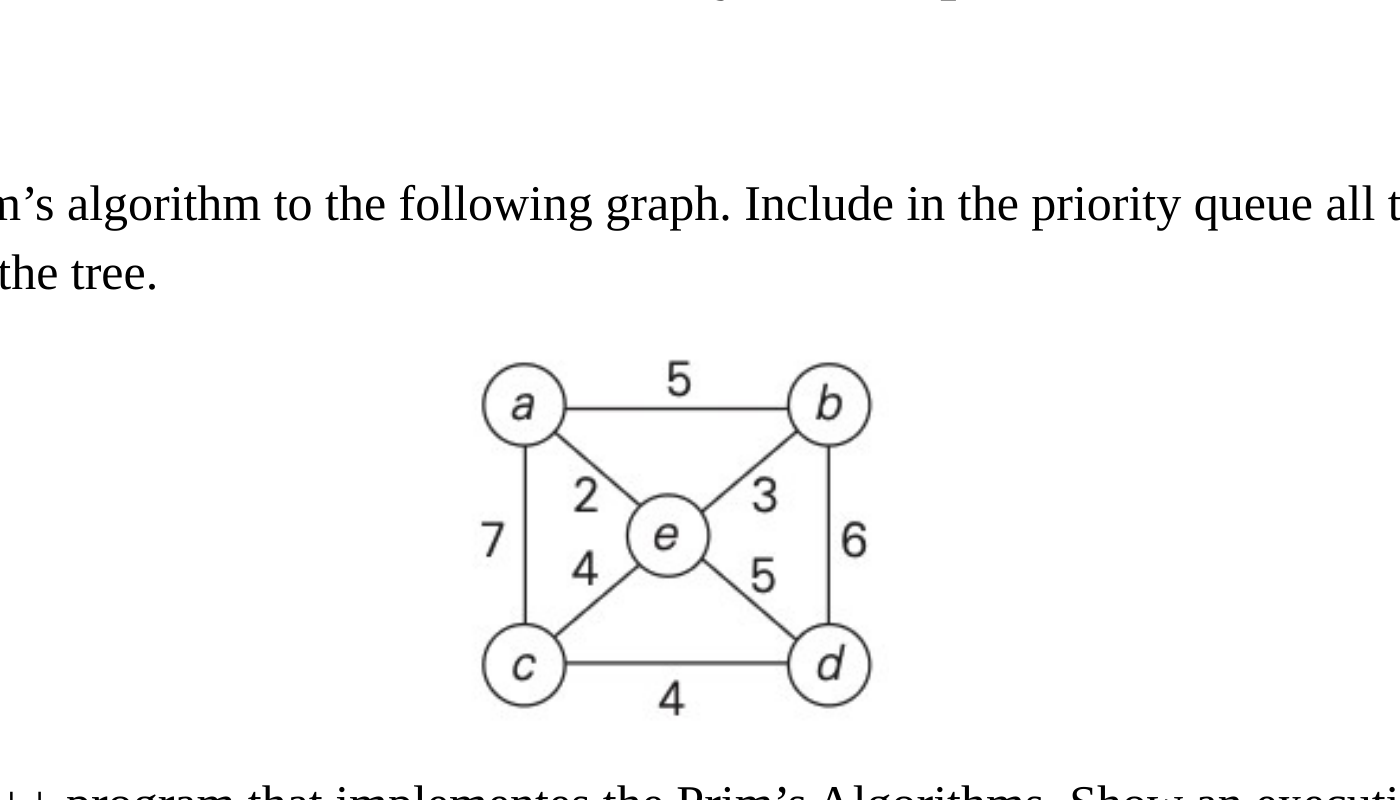
\includegraphics[width=0.48\textwidth]{figures/graph_ex1.png}
    \caption{Original input graph for Exercise 1 from Assignment 09.}
    \label{fig:orig_prim}
\end{figure}

\subsection{My Handwritten Step-by-Step Resolution}
In Figure~\ref{fig:handwritten_prim}, I present my complete manual step-by-step resolution of Prim's algorithm applied to the graph. In my development, I initialize the tree at root vertex $a$, populate and track the priority queue for all remaining vertices using the formal notation $v(\text{parent}, \text{cost})$, iteratively select the minimum-weight connection, update neighbor labels, and obtain the final minimum spanning tree with a total weight of $W = 13$.

\begin{figure}[H]
    \centering
    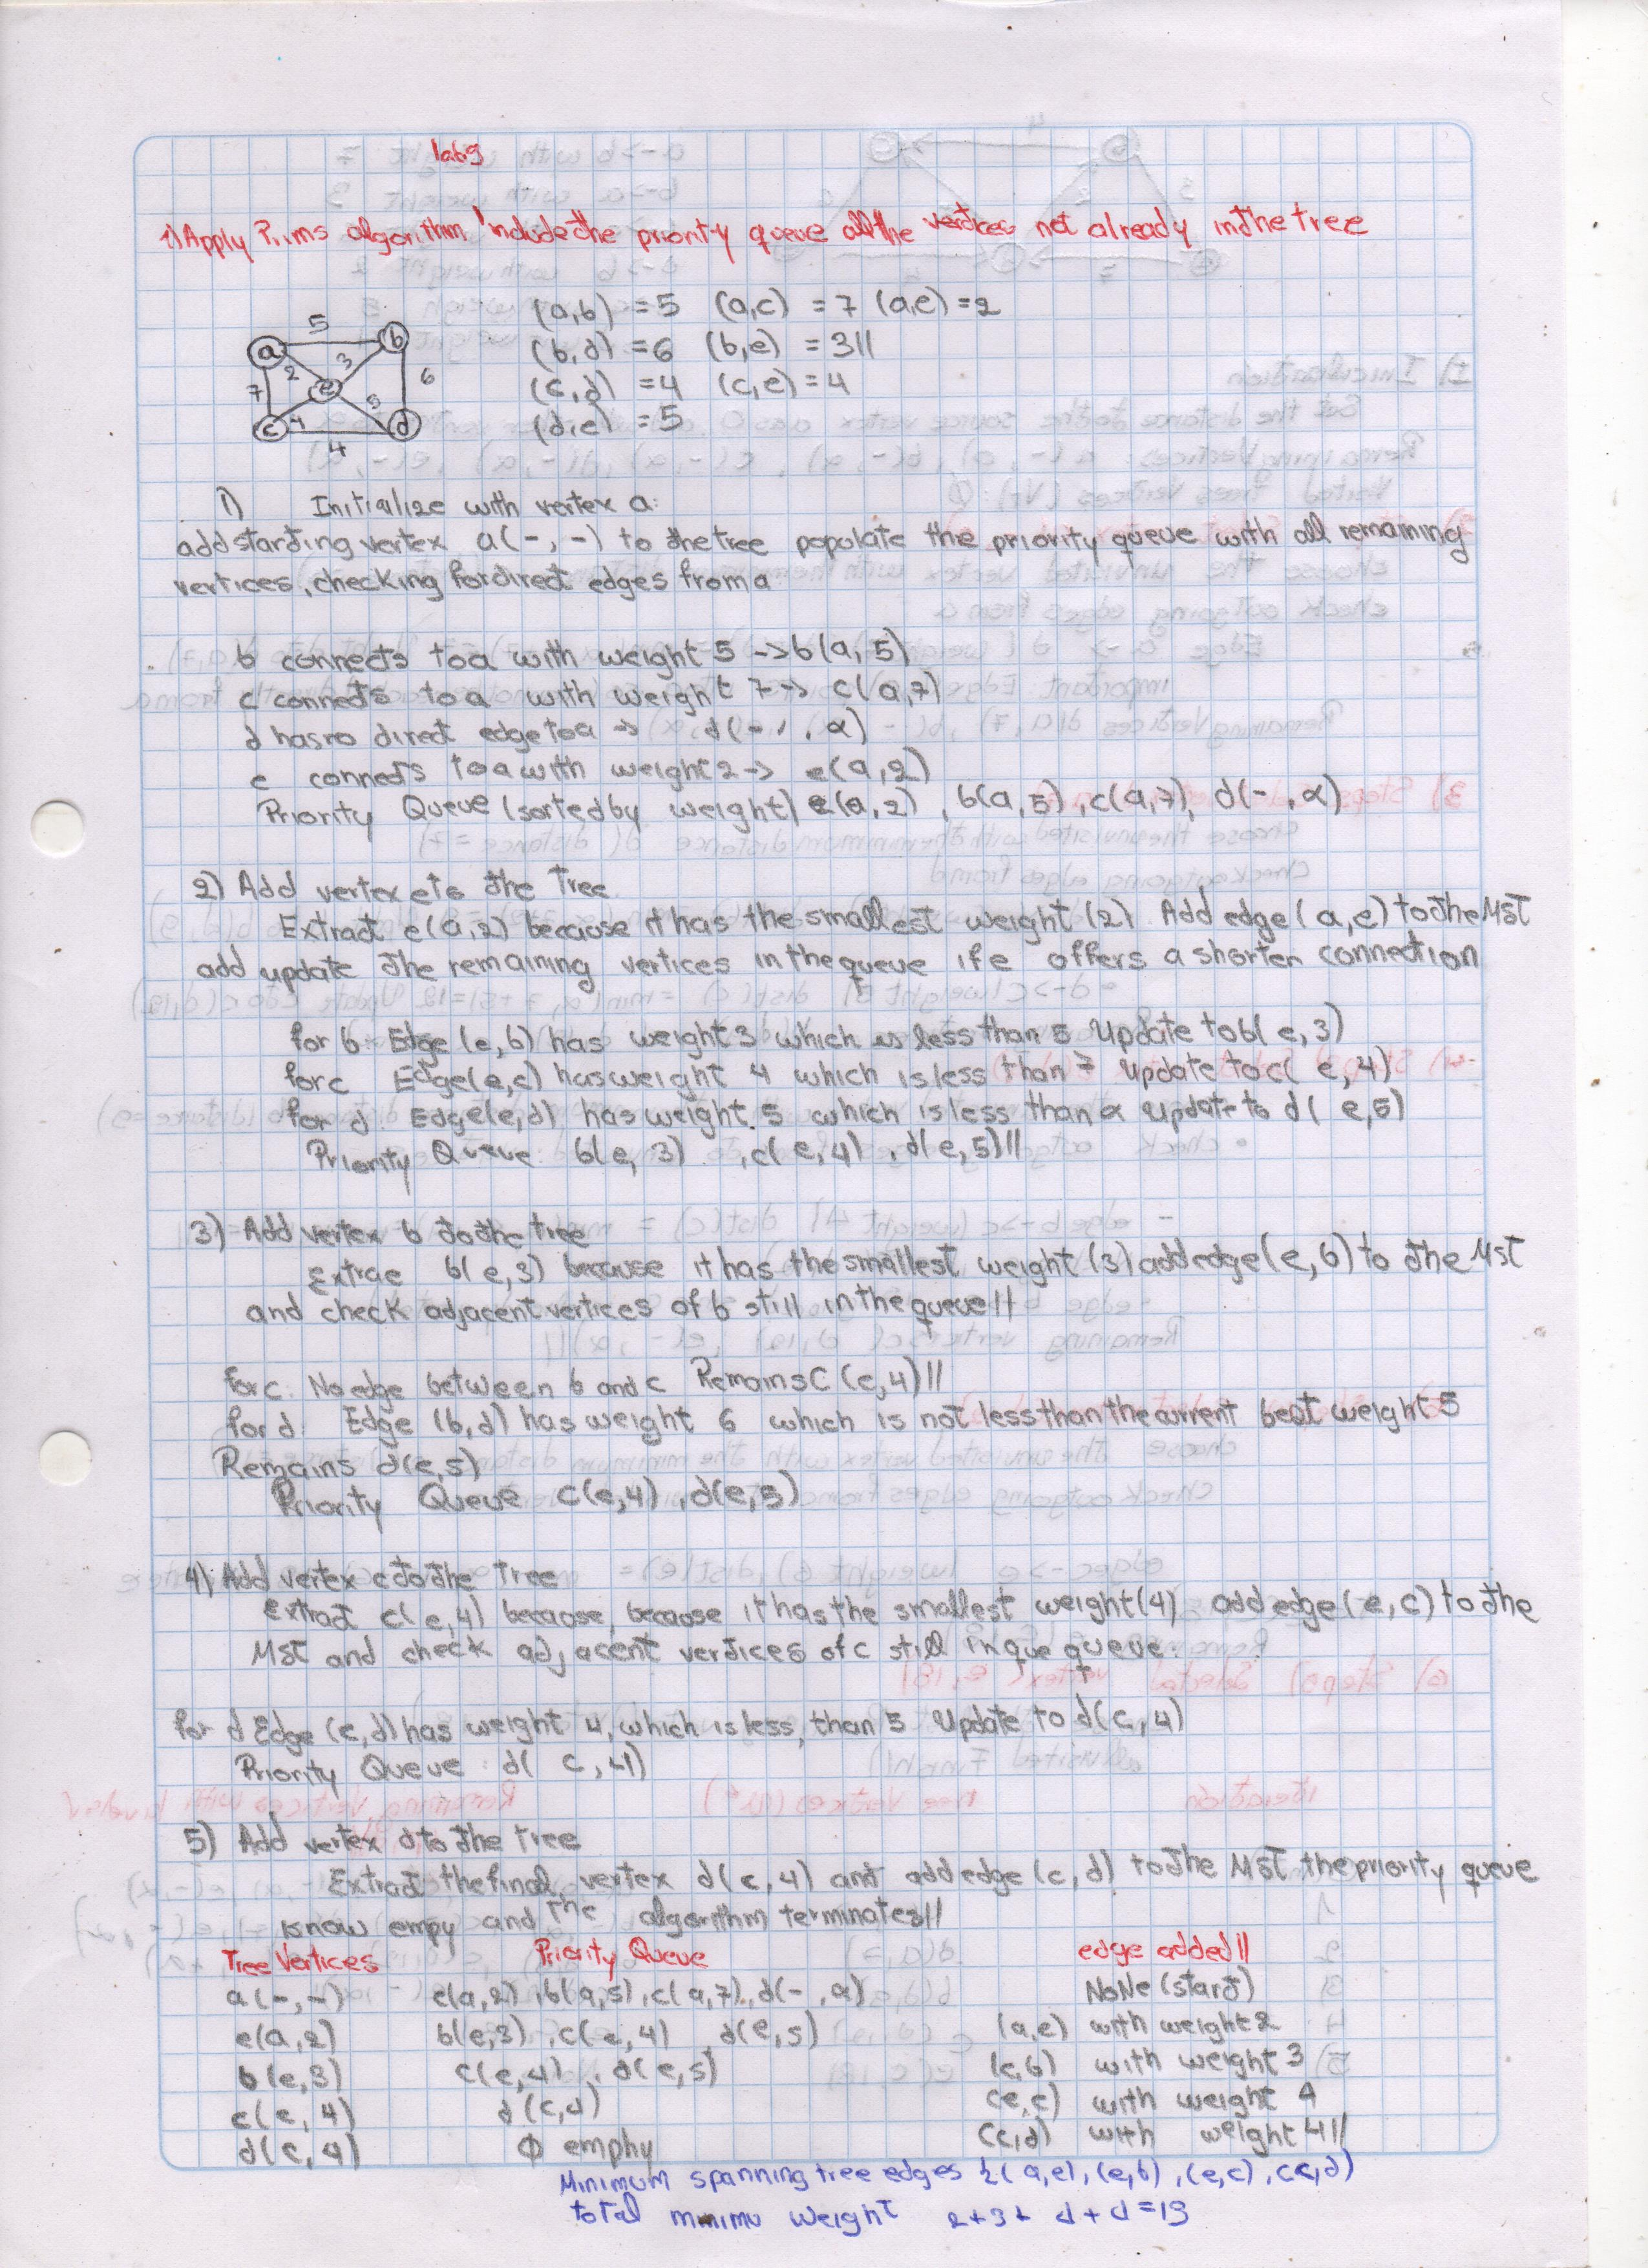
\includegraphics[width=0.75\textwidth]{fotos/001.jpg}
    \caption{My manual step-by-step resolution of Prim's algorithm (Exercise 1).}
    \label{fig:handwritten_prim}
\end{figure}

\subsection{Formal Analytical Verification and Algorithmic Trace}
In addition to my handwritten solution, I provide below the formalized step-by-step trace and vector graph representations to document the exact transitions at each iteration following standard textbook conventions (Levitin, Chapter 9).

The tree is initialized at vertex $a$ ($V_T = \{a\}$). The priority queue holds all candidate vertices $V \setminus V_T$, formatted using the standard notation $v(\text{parent}, \text{key})$.

\begin{table}[H]
\centering
\caption{Complete trace of Prim's algorithm starting at vertex $a$.}
\label{tab:prim_trace}
\begin{tabular}{c p{3.2cm} p{2.6cm} c p{6.4cm}}
\toprule
\textbf{Step} & \textbf{Added Vertex} & \textbf{MST Edge} & \textbf{Weight} & \textbf{Priority Queue ($V \setminus V_T$)} \\
\midrule
0 & Initialization: $a(-, 0)$ & --- & --- & $b(a, 5), \; c(a, 7), \; d(-, \infty), \; \mathbf{e(a, 2)}$ \\
\addlinespace
1 & $e(a, 2)$ & $(a, e)$ & 2 & $\mathbf{b(e, 3)}, \; c(e, 4), \; d(e, 5)$ \\
\addlinespace
2 & $b(e, 3)$ & $(e, b)$ & 3 & $\mathbf{c(e, 4)}, \; d(e, 5)$ \\
\addlinespace
3 & $c(e, 4)$ & $(e, c)$ & 4 & $\mathbf{d(c, 4)}$ \\
\addlinespace
4 & $d(c, 4)$ & $(c, d)$ & 4 & Empty queue ($\emptyset$). Algorithm terminates. \\
\bottomrule
\end{tabular}
\end{table}

\noindent \textbf{Detailed analytical breakdown of step transitions:}
\begin{itemize}
    \item \textbf{Step 0:} Vertex $a$ is selected as the root. Its incident neighbors are $b$ with weight 5, $c$ with weight 7, and $e$ with weight 2. Vertex $d$ has no direct edge to $a$, so its key remains $\infty$.
    \item \textbf{Step 1:} The queue minimum is $e$ with key 2. Edge $(a, e)$ is incorporated into the tree. Exploring neighbors of $e$:
    \begin{itemize}
        \item For $b$: $w(e, b) = 3 < 5$, updated to $b(e, 3)$.
        \item For $c$: $w(e, c) = 4 < 7$, updated to $c(e, 4)$.
        \item For $d$: $w(e, d) = 5 < \infty$, updated to $d(e, 5)$.
    \end{itemize}
    \item \textbf{Step 2:} Minimum is $b$ with key 3. Edge $(e, b)$ is added. Checking edge $(b, d) = 6 > 5$, so the key of $d$ is retained as 5.
    \item \textbf{Step 3:} Minimum is $c$ with key 4. Edge $(e, c)$ is added. Evaluating $(c, d) = 4 < 5$, key of $d$ is relaxed to $d(c, 4)$.
    \item \textbf{Step 4:} Final vertex in queue is $d$ with key 4. Edge $(c, d)$ is added. The queue is now empty.
\end{itemize}

\subsection{Resulting Minimum Spanning Tree and Total Cost}
The generated Minimum Spanning Tree $T = (V, E_T)$ consists of the following 4 edges:
\begin{equation}
    E_T = \left\{ (a, e), \; (e, b), \; (e, c), \; (c, d) \right\}
\end{equation}
The total weight of the MST is:
\begin{equation}
    W(T) = w(a, e) + w(e, b) + w(e, c) + w(c, d) = 2 + 3 + 4 + 4 = \mathbf{13}
\end{equation}

\begin{figure}[H]
    \centering
    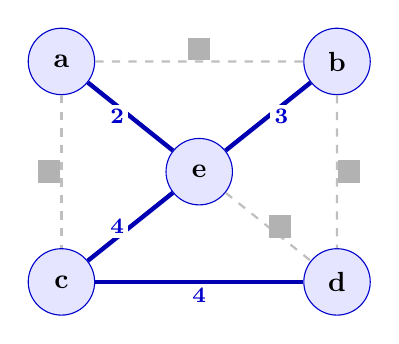
\begin{tikzpicture}[scale=1.4, auto]
        \node[mstvertex] (a) at (0, 2) {a};
        \node[mstvertex] (b) at (2.5, 2) {b};
        \node[mstvertex] (c) at (0, 0) {c};
        \node[mstvertex] (d) at (2.5, 0) {d};
        \node[mstvertex] (e) at (1.25, 1) {e};

        % Discarded edges (gray dashed)
        \draw[edge, dashed, gray!50] (a) -- node[weight, gray!60, above] {5} (b);
        \draw[edge, dashed, gray!50] (a) -- node[weight, gray!60, left] {7} (c);
        \draw[edge, dashed, gray!50] (b) -- node[weight, gray!60, right] {6} (d);
        \draw[edge, dashed, gray!50] (e) -- node[weight, gray!60, right] {5} (d);

        % MST edges (thick solid blue)
        \draw[mstedge] (e) -- node[weight, text=blue!80!black, left] {2} (a);
        \draw[mstedge] (e) -- node[weight, text=blue!80!black, right] {3} (b);
        \draw[mstedge] (e) -- node[weight, text=blue!80!black, left] {4} (c);
        \draw[mstedge] (c) -- node[weight, text=blue!80!black, below] {4} (d);
    \end{tikzpicture}
    \caption{Resulting Minimum Spanning Tree (MST). Solid blue edges indicate members of $T$ ($W = 13$).}
    \label{fig:mst_result}
\end{figure}

\newpage

% ==============================================================================
\section{Exercise 2: C / C++ Implementation of Prim's Algorithm}
% ==============================================================================

To implement the algorithm programmatically, I developed two complete solutions in directory \texttt{ejercicio\_1\_2\_prim/}:
\begin{itemize}
    \item \texttt{prim.c}: My implementation in standard C (C11) with adjacency matrix and priority queue emulation that prints detailed step transitions.
    \item \texttt{prim.cpp}: My implementation in modern C++ (C++17) using standard library containers.
\end{itemize}

\subsection{Architecture and Explained Code Fragments (\texttt{prim.c})}
Rather than examining a monolithic script, the implementation is structured into three clear algorithmic stages detailed below:

\subsubsection{Stage 1: Priority Queue Data Representation and Initialization}
The priority queue and cut tracking are represented using three parallel arrays of size $V = 5$:

\begin{lstlisting}[style=cstyle, caption={State arrays and initialization for Prim's algorithm}]
int parent[V];  // Stores the MST predecessor for each vertex
int key[V];     // Holds the minimum connecting weight to the tree
bool inMST[V];  // Indicates whether a vertex belongs to the tree cut

for (int i = 0; i < V; i++) {
    key[i] = INF;      // Initially, all connection costs are unknown/infinite
    parent[i] = -1;    // No predecessor assigned
    inMST[i] = false;  // No vertex has been included in the tree cut yet
}
key[start_node] = 0;   // Root vertex connection cost is set to 0
inMST[start_node] = true;
\end{lstlisting}

\noindent \textbf{Detailed Explanation:}
\begin{itemize}
    \item \texttt{key[v]}: Represents the priority key in the queue. For any unvisited vertex $v$, it stores the minimum weight of an edge connecting $v$ to any vertex already included in the tree cut $V_T$. Initializing all entries to \texttt{INF} ($999999$) signifies that their connection costs are initially unconstrained.
    \item \texttt{parent[v]}: Tracks the specific tree vertex that provides the minimal-weight connection to $v$. When $v$ is eventually added to the tree, edge $(\text{parent}[v], v)$ forms a valid branch of the MST.
    \item \texttt{inMST[v]}: A boolean membership flag that partitions the graph vertices into the resolved tree cut $V_T$ and the unresolved candidate set $V \setminus V_T$. Setting \texttt{key[start\_node] = 0} ensures that the starting vertex $a$ is greedily selected first.
\end{itemize}

\subsubsection{Stage 2: Greedy Selection of Minimal Cut Edge (\texttt{extract\_min})}
At each step, the algorithm must extract the vertex from the candidate set with the smallest tentative connection cost:

\begin{lstlisting}[style=cstyle, caption={Linear-scan minimum extraction from candidate cut}]
int extract_min(int key[], bool inMST[]) {
    int min_val = INF, min_index = -1;
    for (int v = 0; v < V; v++) {
        if (!inMST[v] && key[v] < min_val) {
            min_val = key[v];
            min_index = v;
        }
    }
    return min_index; // Returns vertex index with the global minimum key
}
\end{lstlisting}

\noindent \textbf{Detailed Explanation:}
This routine directly embodies the \textbf{Greedy Choice Property}. It iterates strictly across unvisited vertices (\texttt{!inMST[v]}) to find the vertex with the minimal \texttt{key[v]}. For small to medium dense graphs, an array-based $O(V)$ scan offers outstanding cache locality and zero memory overhead compared to a binary min-heap.

\subsubsection{Stage 3: Edge Relaxation and Queue Key Updates}
Once the minimal vertex $u$ is added to the tree cut (\texttt{inMST[u] = true}), its outgoing incident edges are inspected to update the priority queue:

\begin{lstlisting}[style=cstyle, caption={Edge relaxation and neighbor key updates}]
for (int v = 0; v < V; v++) {
    if (graph[u][v] != 0 && !inMST[v]) {
        // If edge (u, v) provides a cheaper connection to the tree
        if (graph[u][v] < key[v]) {
            key[v] = graph[u][v];  // Decrease priority key of v
            parent[v] = u;         // Update predecessor to u
        }
    }
}
\end{lstlisting}

\noindent \textbf{Detailed Explanation:}
For every neighbor $v$ that remains outside the tree cut (\texttt{!inMST[v]}), the code tests whether connecting $v$ through the newly added vertex $u$ offers a lower cost than its currently recorded best option (\texttt{graph[u][v] < key[v]}). If true, the key is decreased and $u$ is designated as $v$'s new parent. This ensures the priority queue accurately reflects the closest frontier to the expanding tree.

\subsection{Program Compilation and Terminal Execution Outputs}
The implementations compile cleanly with GCC and G++ using standard flags:
\begin{lstlisting}[style=terminalstyle]
gcc -Wall -Wextra -O2 prim.c -o prim_c.exe
g++ -Wall -Wextra -O2 prim.cpp -o prim_cpp.exe
\end{lstlisting}

Figures~\ref{fig:out_prim_c} and~\ref{fig:out_prim_cpp} display the actual terminal execution output captures obtained from running \texttt{prim\_c.exe} and \texttt{prim\_cpp.exe}, validating each transition against the manual derivation:

\begin{figure}[H]
    \centering
    \begin{minipage}{0.48\textwidth}
        \centering
        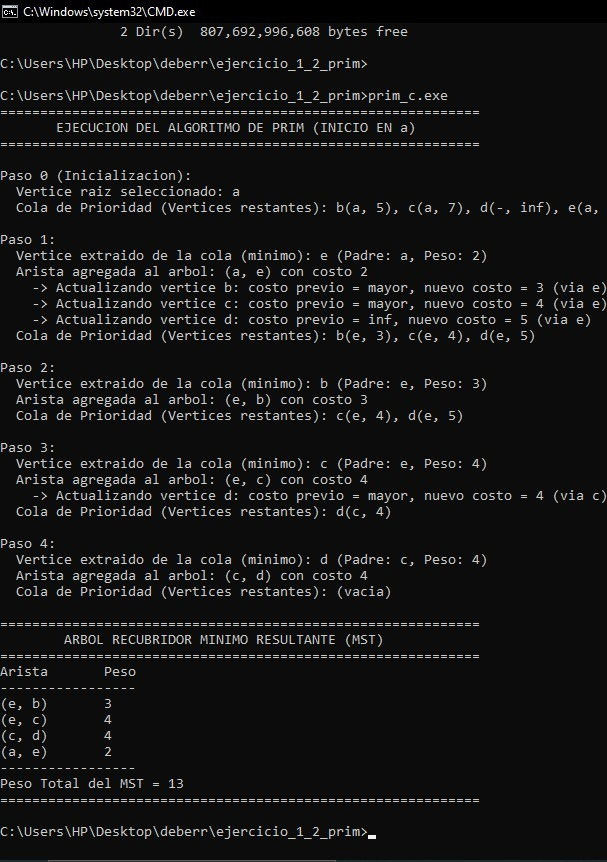
\includegraphics[width=\textwidth]{fotos/salida-prime_c.jpeg}
        \caption{Terminal execution capture of \texttt{prim\_c.exe} (C implementation).}
        \label{fig:out_prim_c}
    \end{minipage}
    \hfill
    \begin{minipage}{0.48\textwidth}
        \centering
        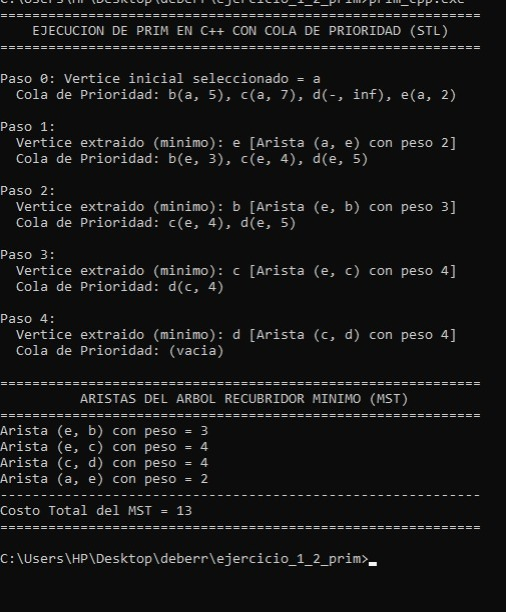
\includegraphics[width=\textwidth]{fotos/salida-prime_cpp.jpeg}
        \caption{Terminal execution capture of \texttt{prim\_cpp.exe} (C++ STL implementation).}
        \label{fig:out_prim_cpp}
    \end{minipage}
\end{figure}

\newpage

% ==============================================================================
\section{Exercise 3: Dijkstra's Algorithm (Step-by-Step Resolution)}
% ==============================================================================

\subsection{Instance 3.a: Directed Graph}
\textbf{Task:} \textit{Solve (paper and pencil) the following instances of the single-source shortest-paths problem with vertex a as the source using Dijkstra's Algorithm: a.}

Figure~\ref{fig:orig_3a} illustrates the directed graph instance.

\begin{figure}[H]
    \centering
    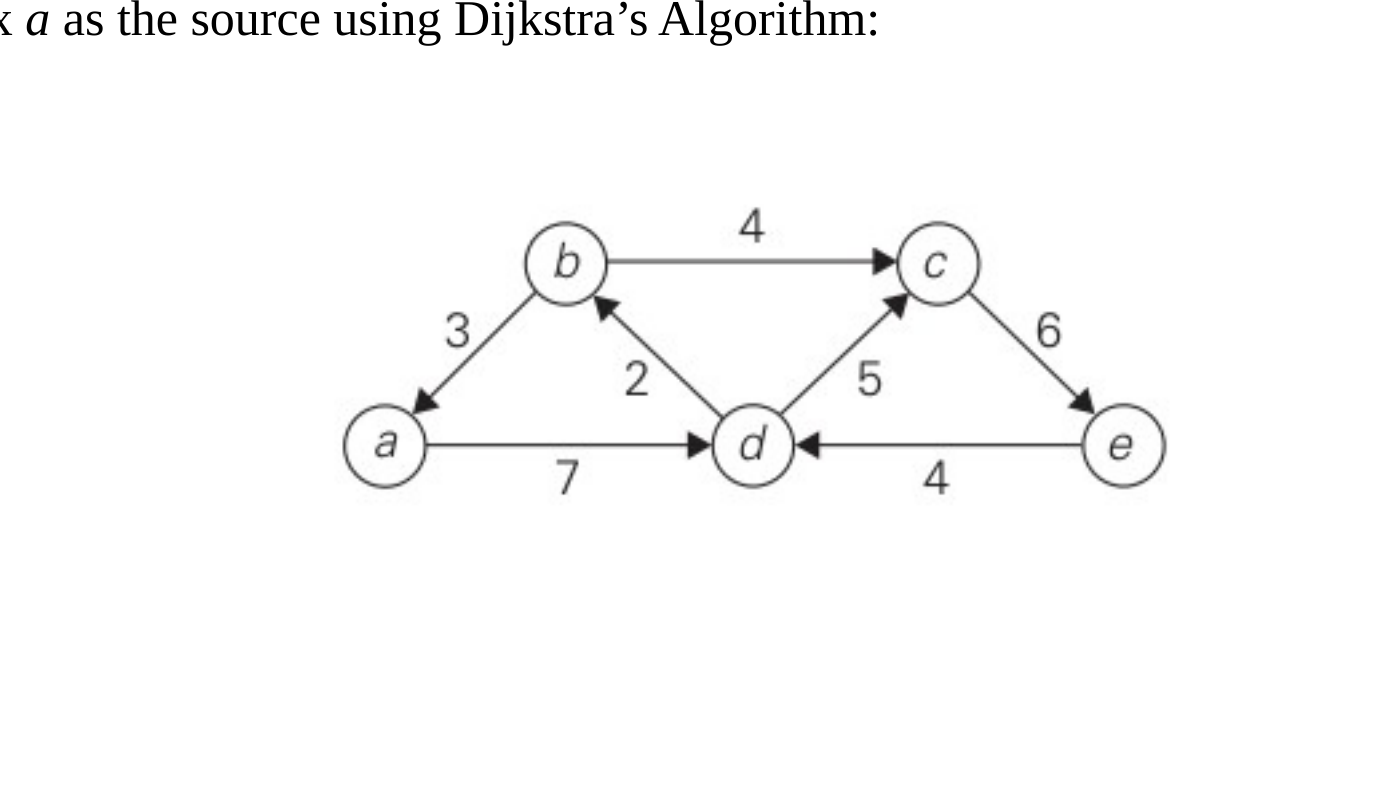
\includegraphics[width=0.62\textwidth]{figures/graph_ex3a.png}
    \caption{Original graph for Instance 3.a from Assignment 09.}
    \label{fig:orig_3a}
\end{figure}

\subsubsection{My Handwritten Step-by-Step Resolution}
Figure~\ref{fig:handwritten_3a} presents my complete paper-and-pencil resolution of Dijkstra's algorithm for Instance 3.a. In this manual derivation, I detail the initialization at source $a$, the unvisited vertex evaluations, the edge relaxations honoring arrow directions, and the progressive computation of shortest paths.

\begin{figure}[H]
    \centering
    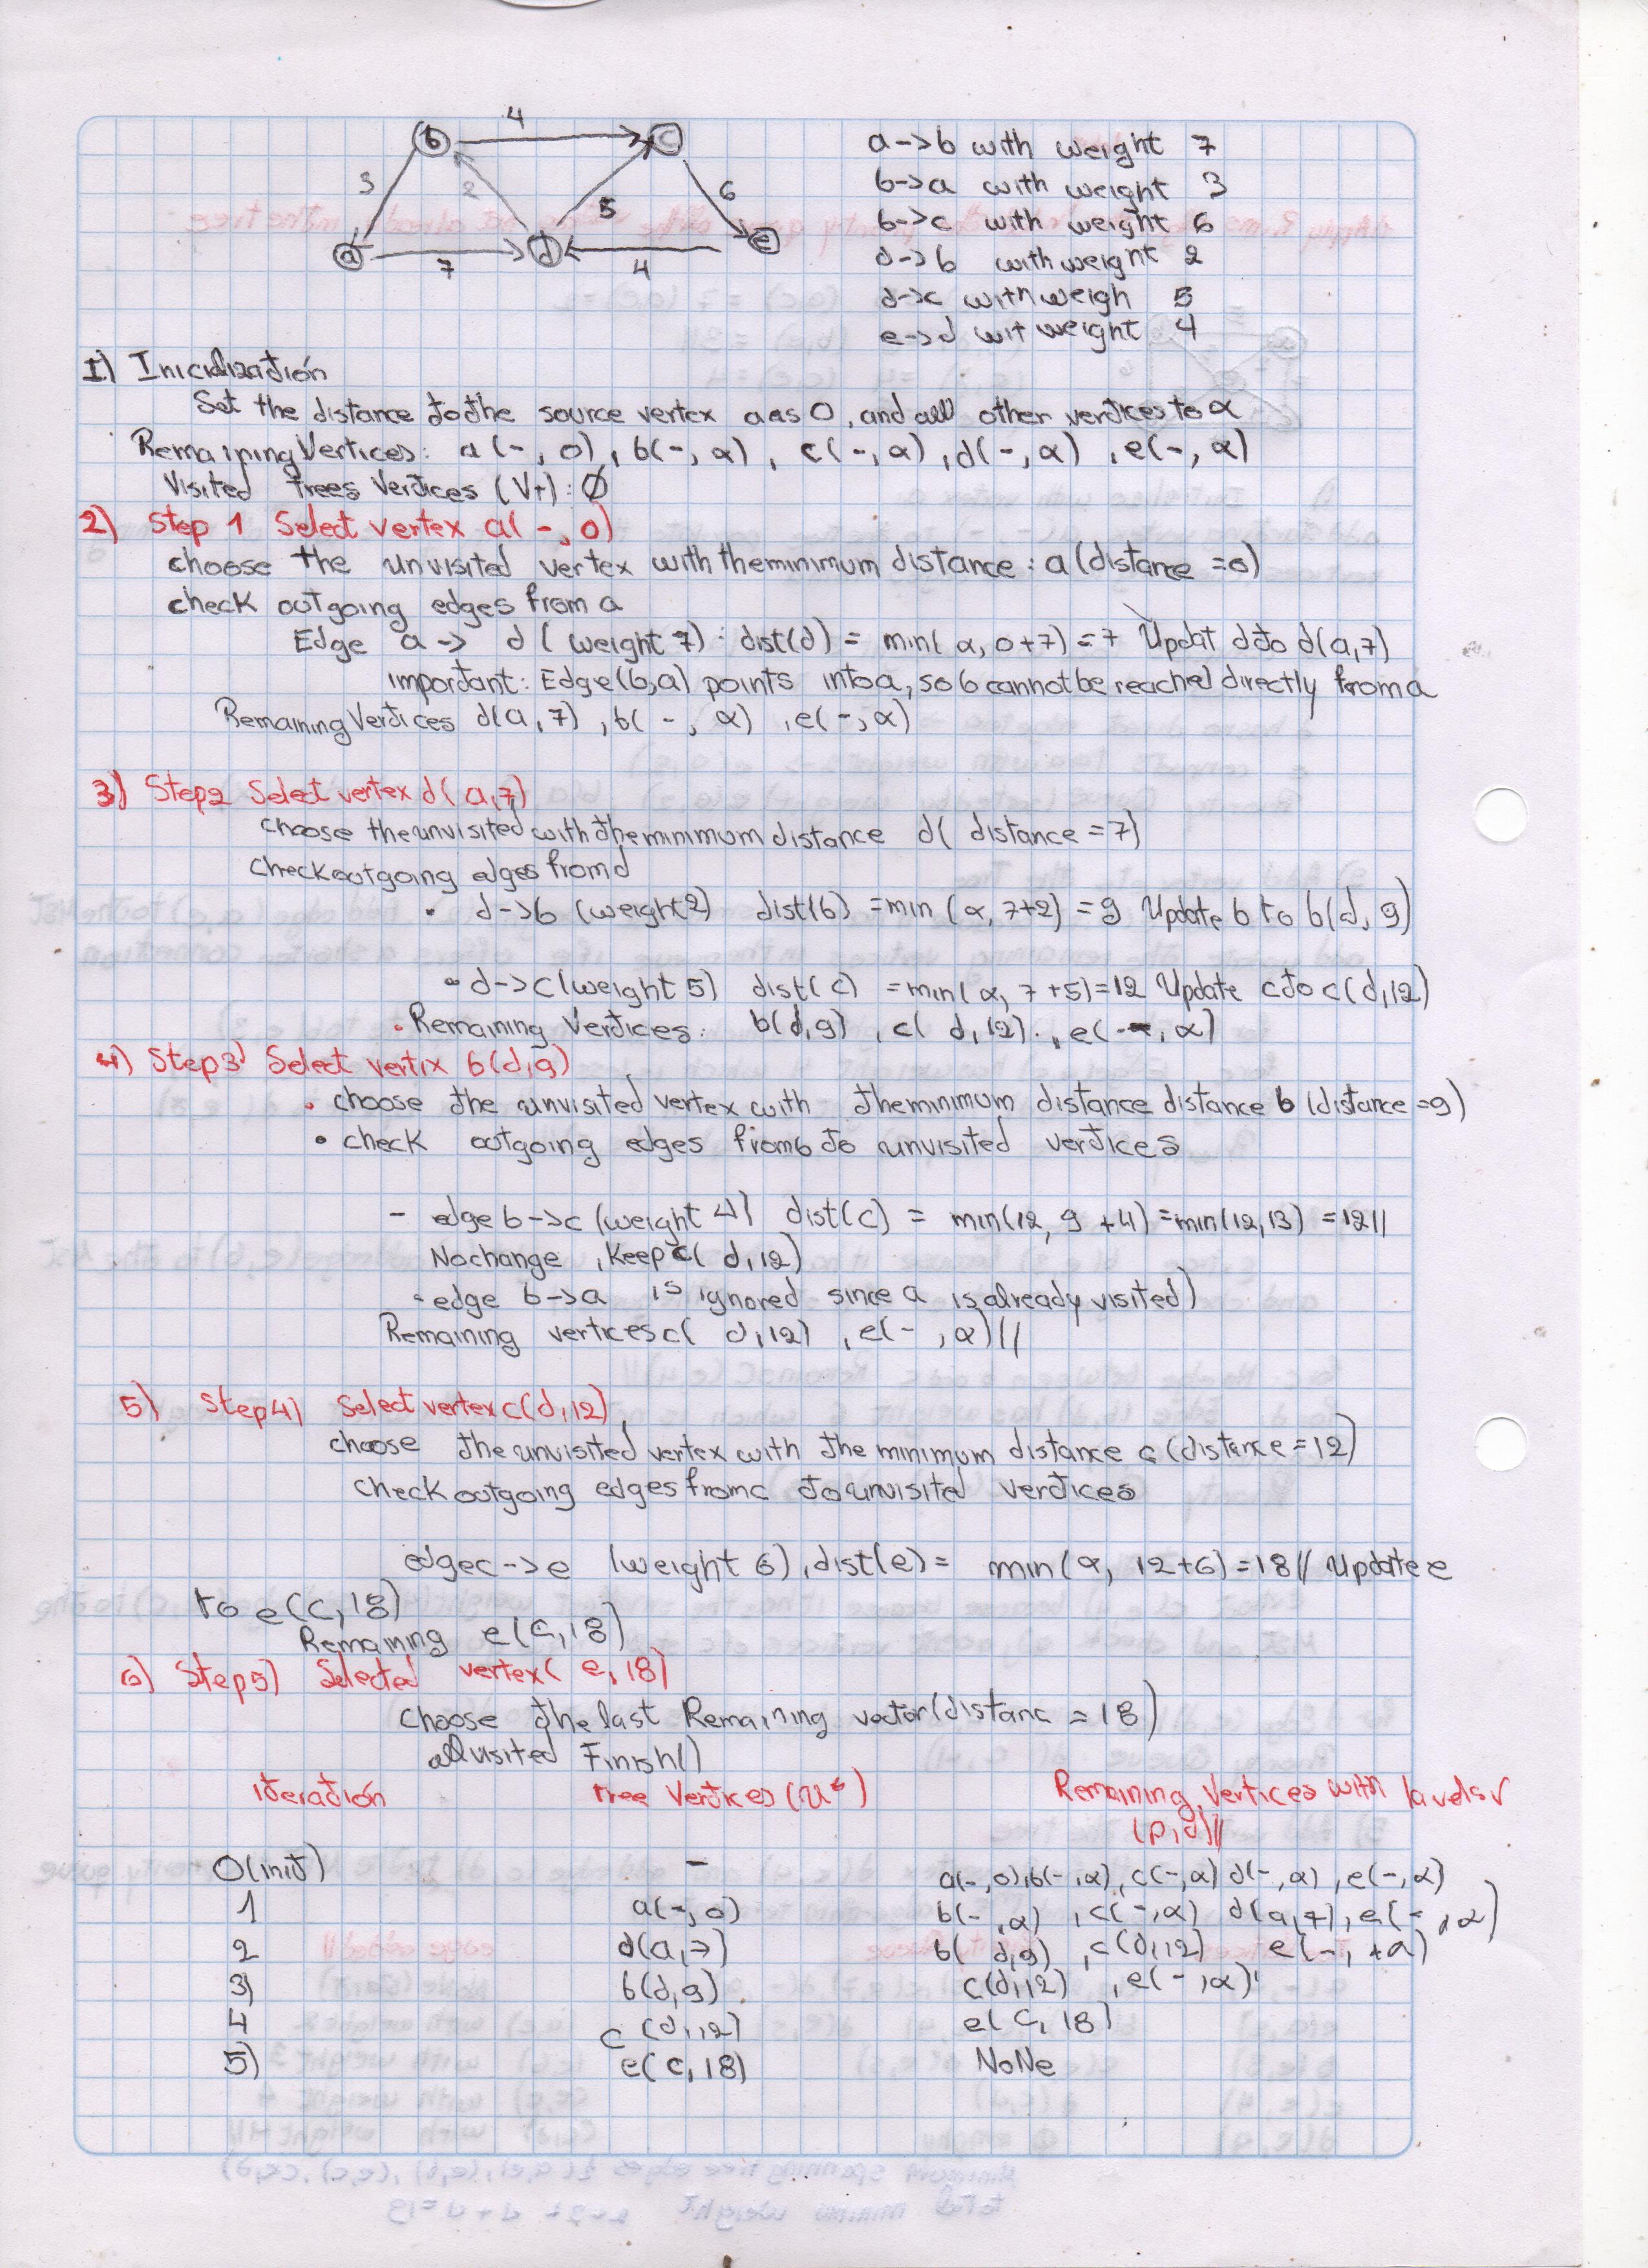
\includegraphics[width=0.75\textwidth]{fotos/3a.jpg}
    \caption{My manual step-by-step resolution of Dijkstra's algorithm for Instance 3.a.}
    \label{fig:handwritten_3a}
\end{figure}

\subsubsection{Edge Directionality Analysis}
This graph is a directed graph (digraph). Inspecting the arrowheads:
\begin{itemize}
    \item $a \rightarrow d$ (weight 7): the only directed edge originating from source vertex $a$.
    \item $b \rightarrow a$ (weight 3): directed towards $a$ (does not allow traveling from $a$ directly to $b$).
    \item $d \rightarrow b$ (weight 2): connects $d$ to $b$.
    \item $b \rightarrow c$ (weight 4): connects $b$ to $c$.
    \item $d \rightarrow c$ (weight 5): connects $d$ to $c$.
    \item $c \rightarrow e$ (weight 6): connects $c$ to $e$.
    \item $e \rightarrow d$ (weight 4): connects $e$ to $d$.
\end{itemize}

\subsubsection{Step-by-Step Execution Trace (Source a)}

\begin{table}[H]
\centering
\caption{Dijkstra's execution trace for Instance 3.a.}
\label{tab:dijkstra_3a_trace}
\begin{tabular}{c p{3.2cm} p{7.2cm} p{3.5cm}}
\toprule
\textbf{Step} & \textbf{Added Vertex $V_T$} & \textbf{Priority Queue ($V \setminus V_T$)} & \textbf{Greedy Operation} \\
\midrule
0 & $a(-, 0)$ & $\mathbf{d(a, 7)}, \; b(-, \infty), \; c(-, \infty), \; e(-, \infty)$ & Source added \\
\addlinespace
1 & $d(a, 7)$ & $\mathbf{b(d, 9)}, \; c(d, 12), \; e(-, \infty)$ & Relaxes $d \rightarrow b, d \rightarrow c$ \\
\addlinespace
2 & $b(d, 9)$ & $\mathbf{c(d, 12)}, \; e(-, \infty)$ & $b \rightarrow c$ gives $13 > 12$ (retained) \\
\addlinespace
3 & $c(d, 12)$ & $\mathbf{e(c, 18)}$ & Relaxes $c \rightarrow e$ ($12 + 6 = 18$) \\
\addlinespace
4 & $e(c, 18)$ & $\emptyset$ (Queue empty) & $e \rightarrow d$ ($d \in V_T$, done) \\
\bottomrule
\end{tabular}
\end{table}

\begin{table}[H]
\centering
\caption{Shortest distances and optimal reconstructed paths from source $a$ (Instance 3.a).}
\begin{tabular}{cccc}
\toprule
\textbf{Destination} & \textbf{Distance $d(v)$} & \textbf{Predecessor} & \textbf{Optimal Route} \\
\midrule
$a$ & 0 & --- & $a$ \\
$b$ & 9 & $d$ & $a \rightarrow d \rightarrow b$ \\
$c$ & 12 & $d$ & $a \rightarrow d \rightarrow c$ \\
$d$ & 7 & $a$ & $a \rightarrow d$ \\
$e$ & 18 & $c$ & $a \rightarrow d \rightarrow c \rightarrow e$ \\
\bottomrule
\end{tabular}
\end{table}

\begin{center}
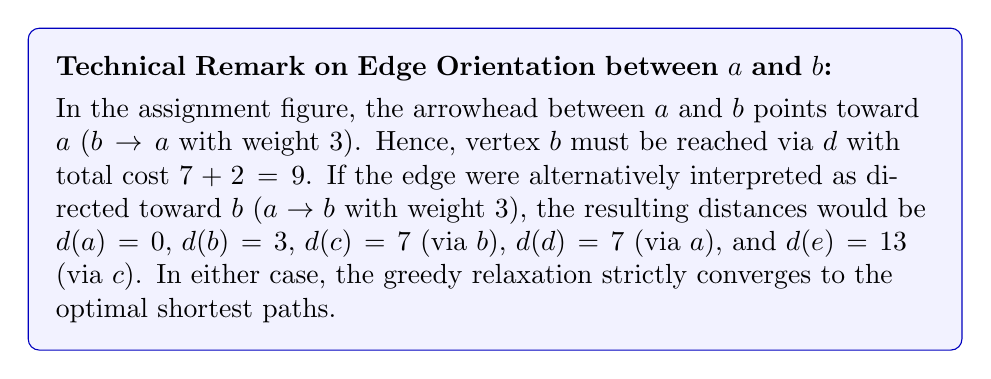
\begin{tikzpicture}
\node[draw=blue!75!black, fill=blue!5!white, rounded corners, inner sep=10pt, text width=0.92\textwidth] {
    \textbf{Technical Remark on Edge Orientation between $a$ and $b$:}\\[0.12cm]
    In the assignment figure, the arrowhead between $a$ and $b$ points toward $a$ ($b \rightarrow a$ with weight 3). Hence, vertex $b$ must be reached via $d$ with total cost $7 + 2 = 9$. If the edge were alternatively interpreted as directed toward $b$ ($a \rightarrow b$ with weight 3), the resulting distances would be $d(a)=0$, $d(b)=3$, $d(c)=7$ (via $b$), $d(d)=7$ (via $a$), and $d(e)=13$ (via $c$). In either case, the greedy relaxation strictly converges to the optimal shortest paths.
};
\end{tikzpicture}
\end{center}

\newpage

\subsection{Instance 3.b: 12-Vertex Undirected Network}
\textbf{Task:} \textit{Solve (paper and pencil) the following instances of the single-source shortest-paths problem with vertex a as the source using Dijkstra's Algorithm: b.}

The graph consists of 12 vertices and 20 undirected weighted edges, shown in Figure~\ref{fig:orig_3b}.

\begin{figure}[H]
    \centering
    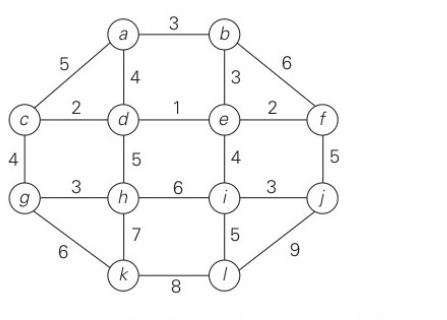
\includegraphics[width=0.68\textwidth]{figures/graph_ex3b.jpeg}
    \caption{Original 12-vertex network for Instance 3.b from Assignment 09.}
    \label{fig:orig_3b}
\end{figure}

\subsubsection{My Handwritten Step-by-Step Resolution}
Figures~\ref{fig:handwritten_3b_p1} and~\ref{fig:handwritten_3b_p2} present my complete manual paper-and-pencil resolution of Dijkstra's algorithm across the 12-vertex network:
\begin{itemize}
    \item \textbf{Part 1 (Figure~\ref{fig:handwritten_3b_p1}):} Network edge inventory, initialization at source vertex $a$, and Iterations 1 through 6 (resolving vertices $a, b, d, c, e, f$).
    \item \textbf{Part 2 (Figure~\ref{fig:handwritten_3b_p2}):} Iterations 7 through 11 (resolving vertices $g, h, i, j, l, k$) and the final destination-by-destination shortest path and cost table.
\end{itemize}

\begin{figure}[H]
    \centering
    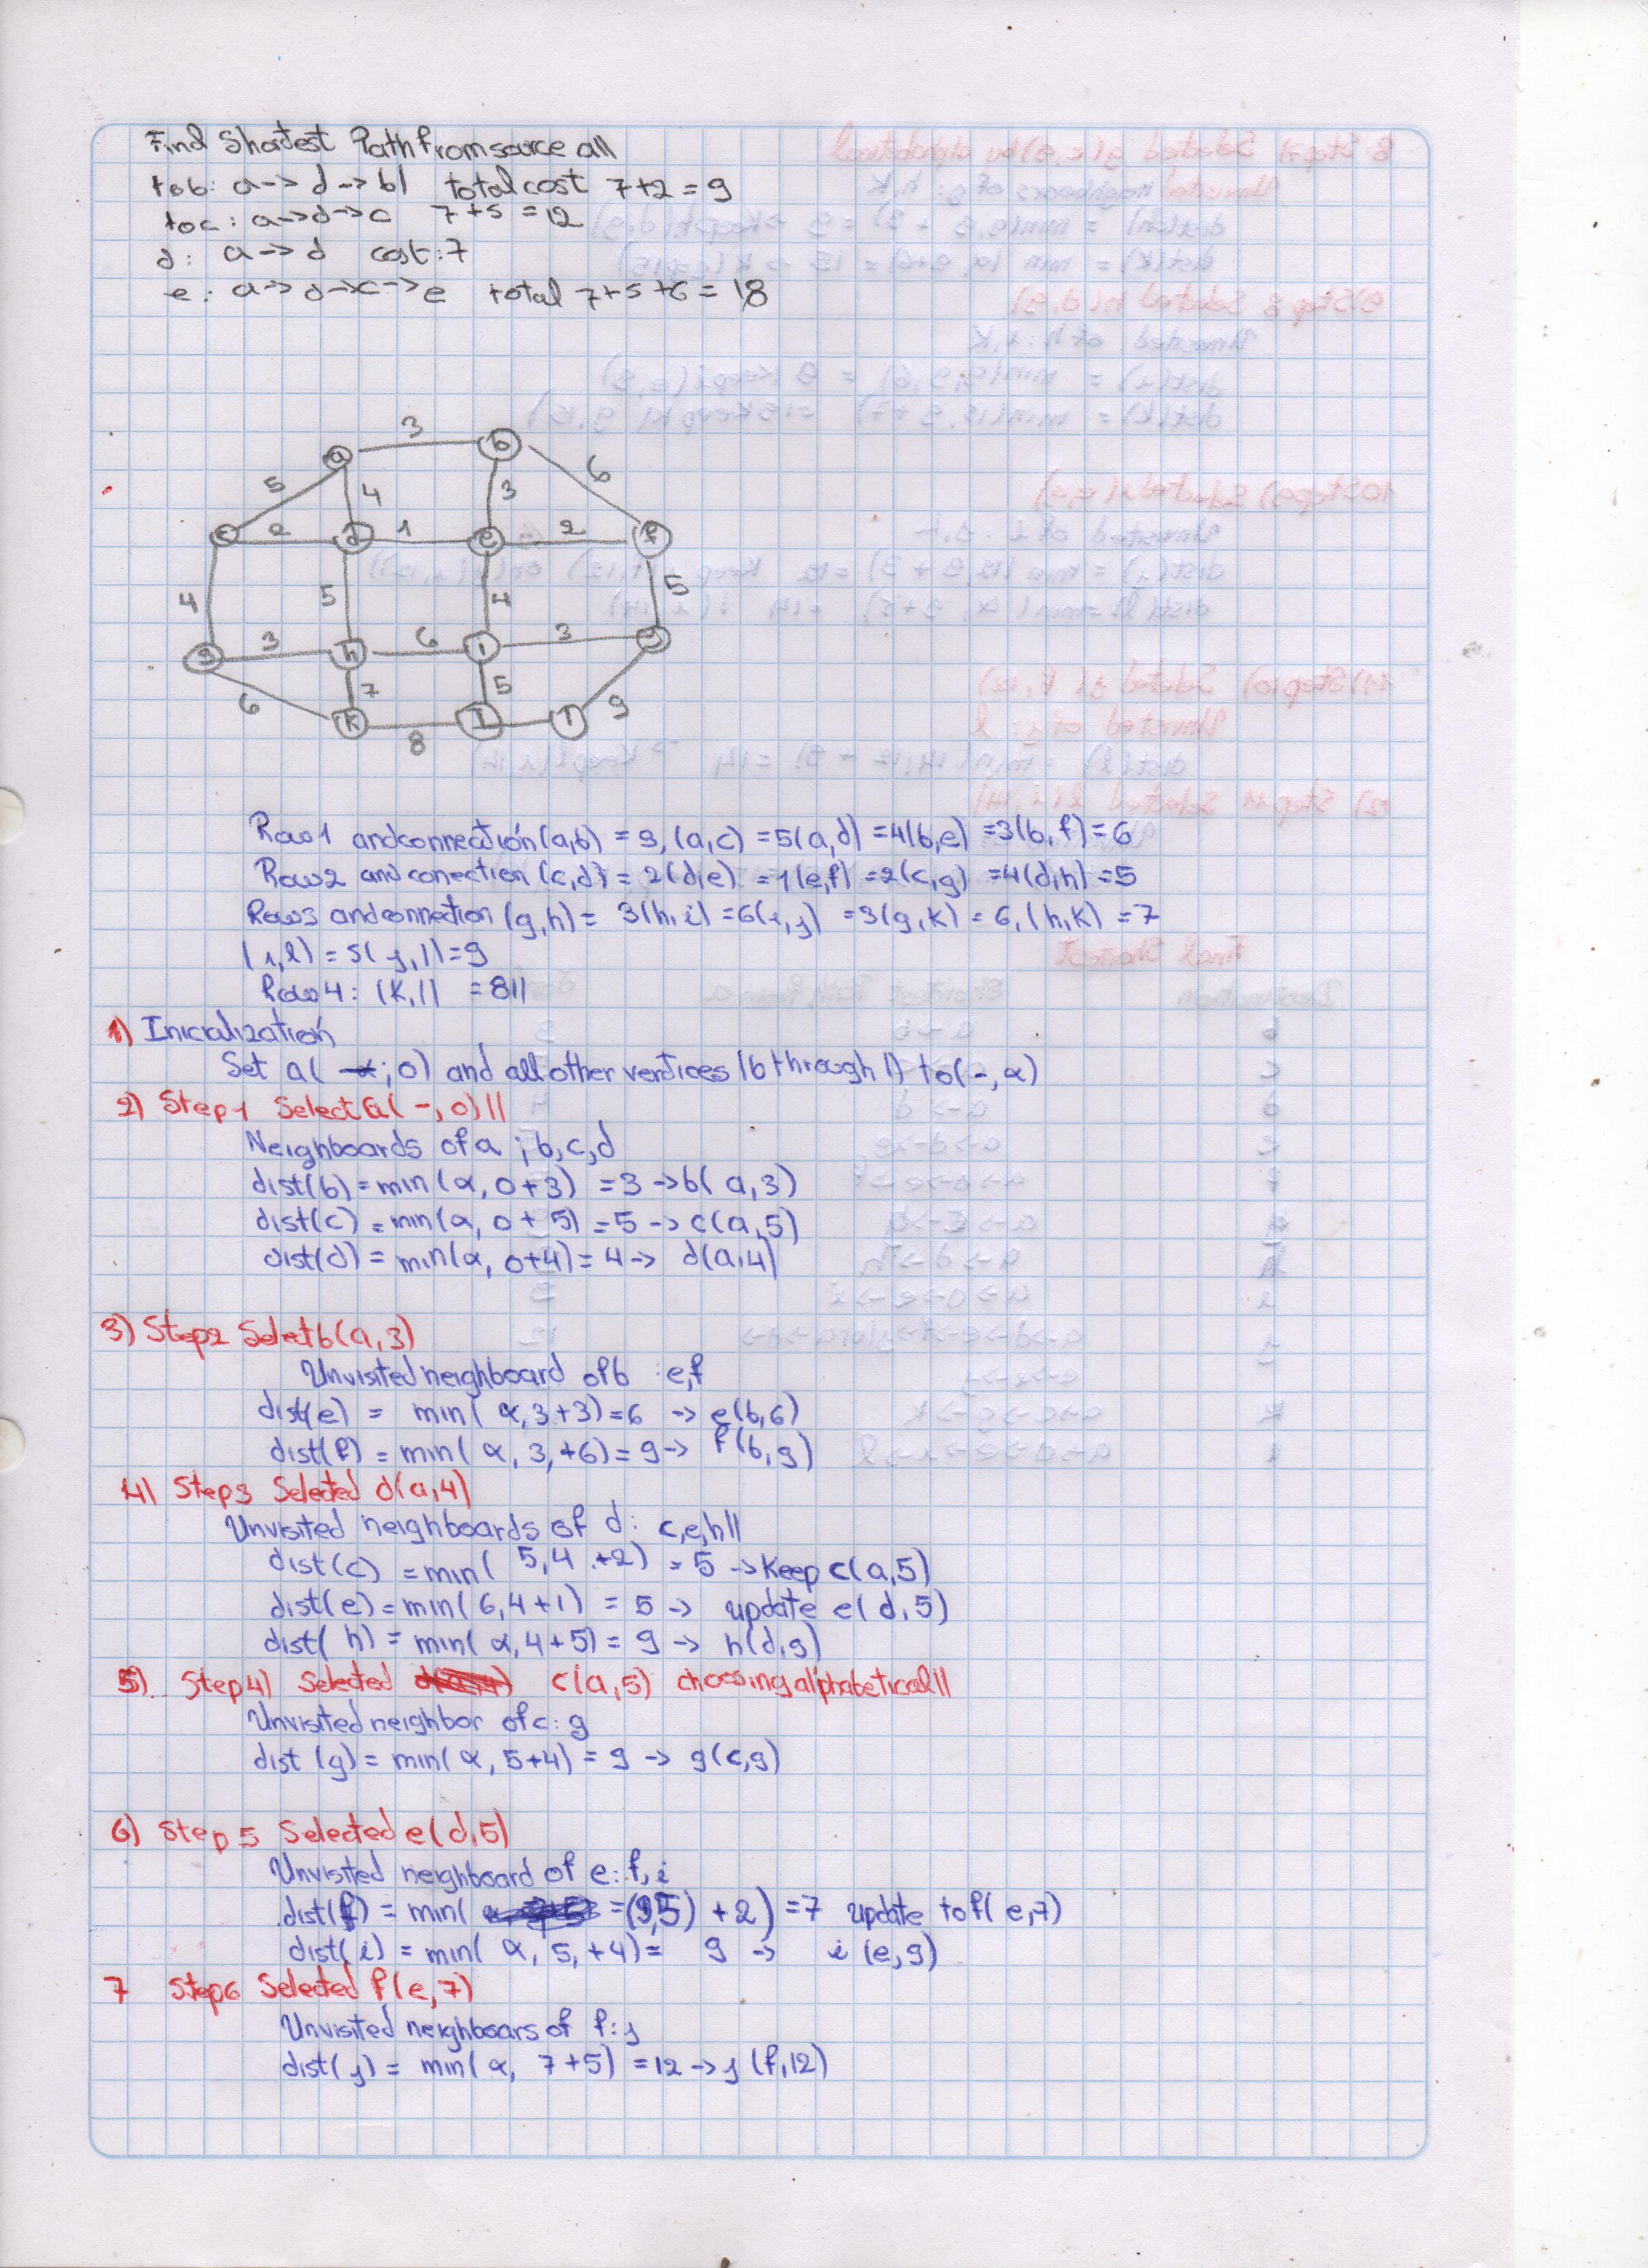
\includegraphics[width=0.75\textwidth]{fotos/3b-parte1.jpg}
    \caption{My manual step-by-step resolution for Instance 3.b (Part 1: Steps 1--6).}
    \label{fig:handwritten_3b_p1}
\end{figure}

\begin{figure}[H]
    \centering
    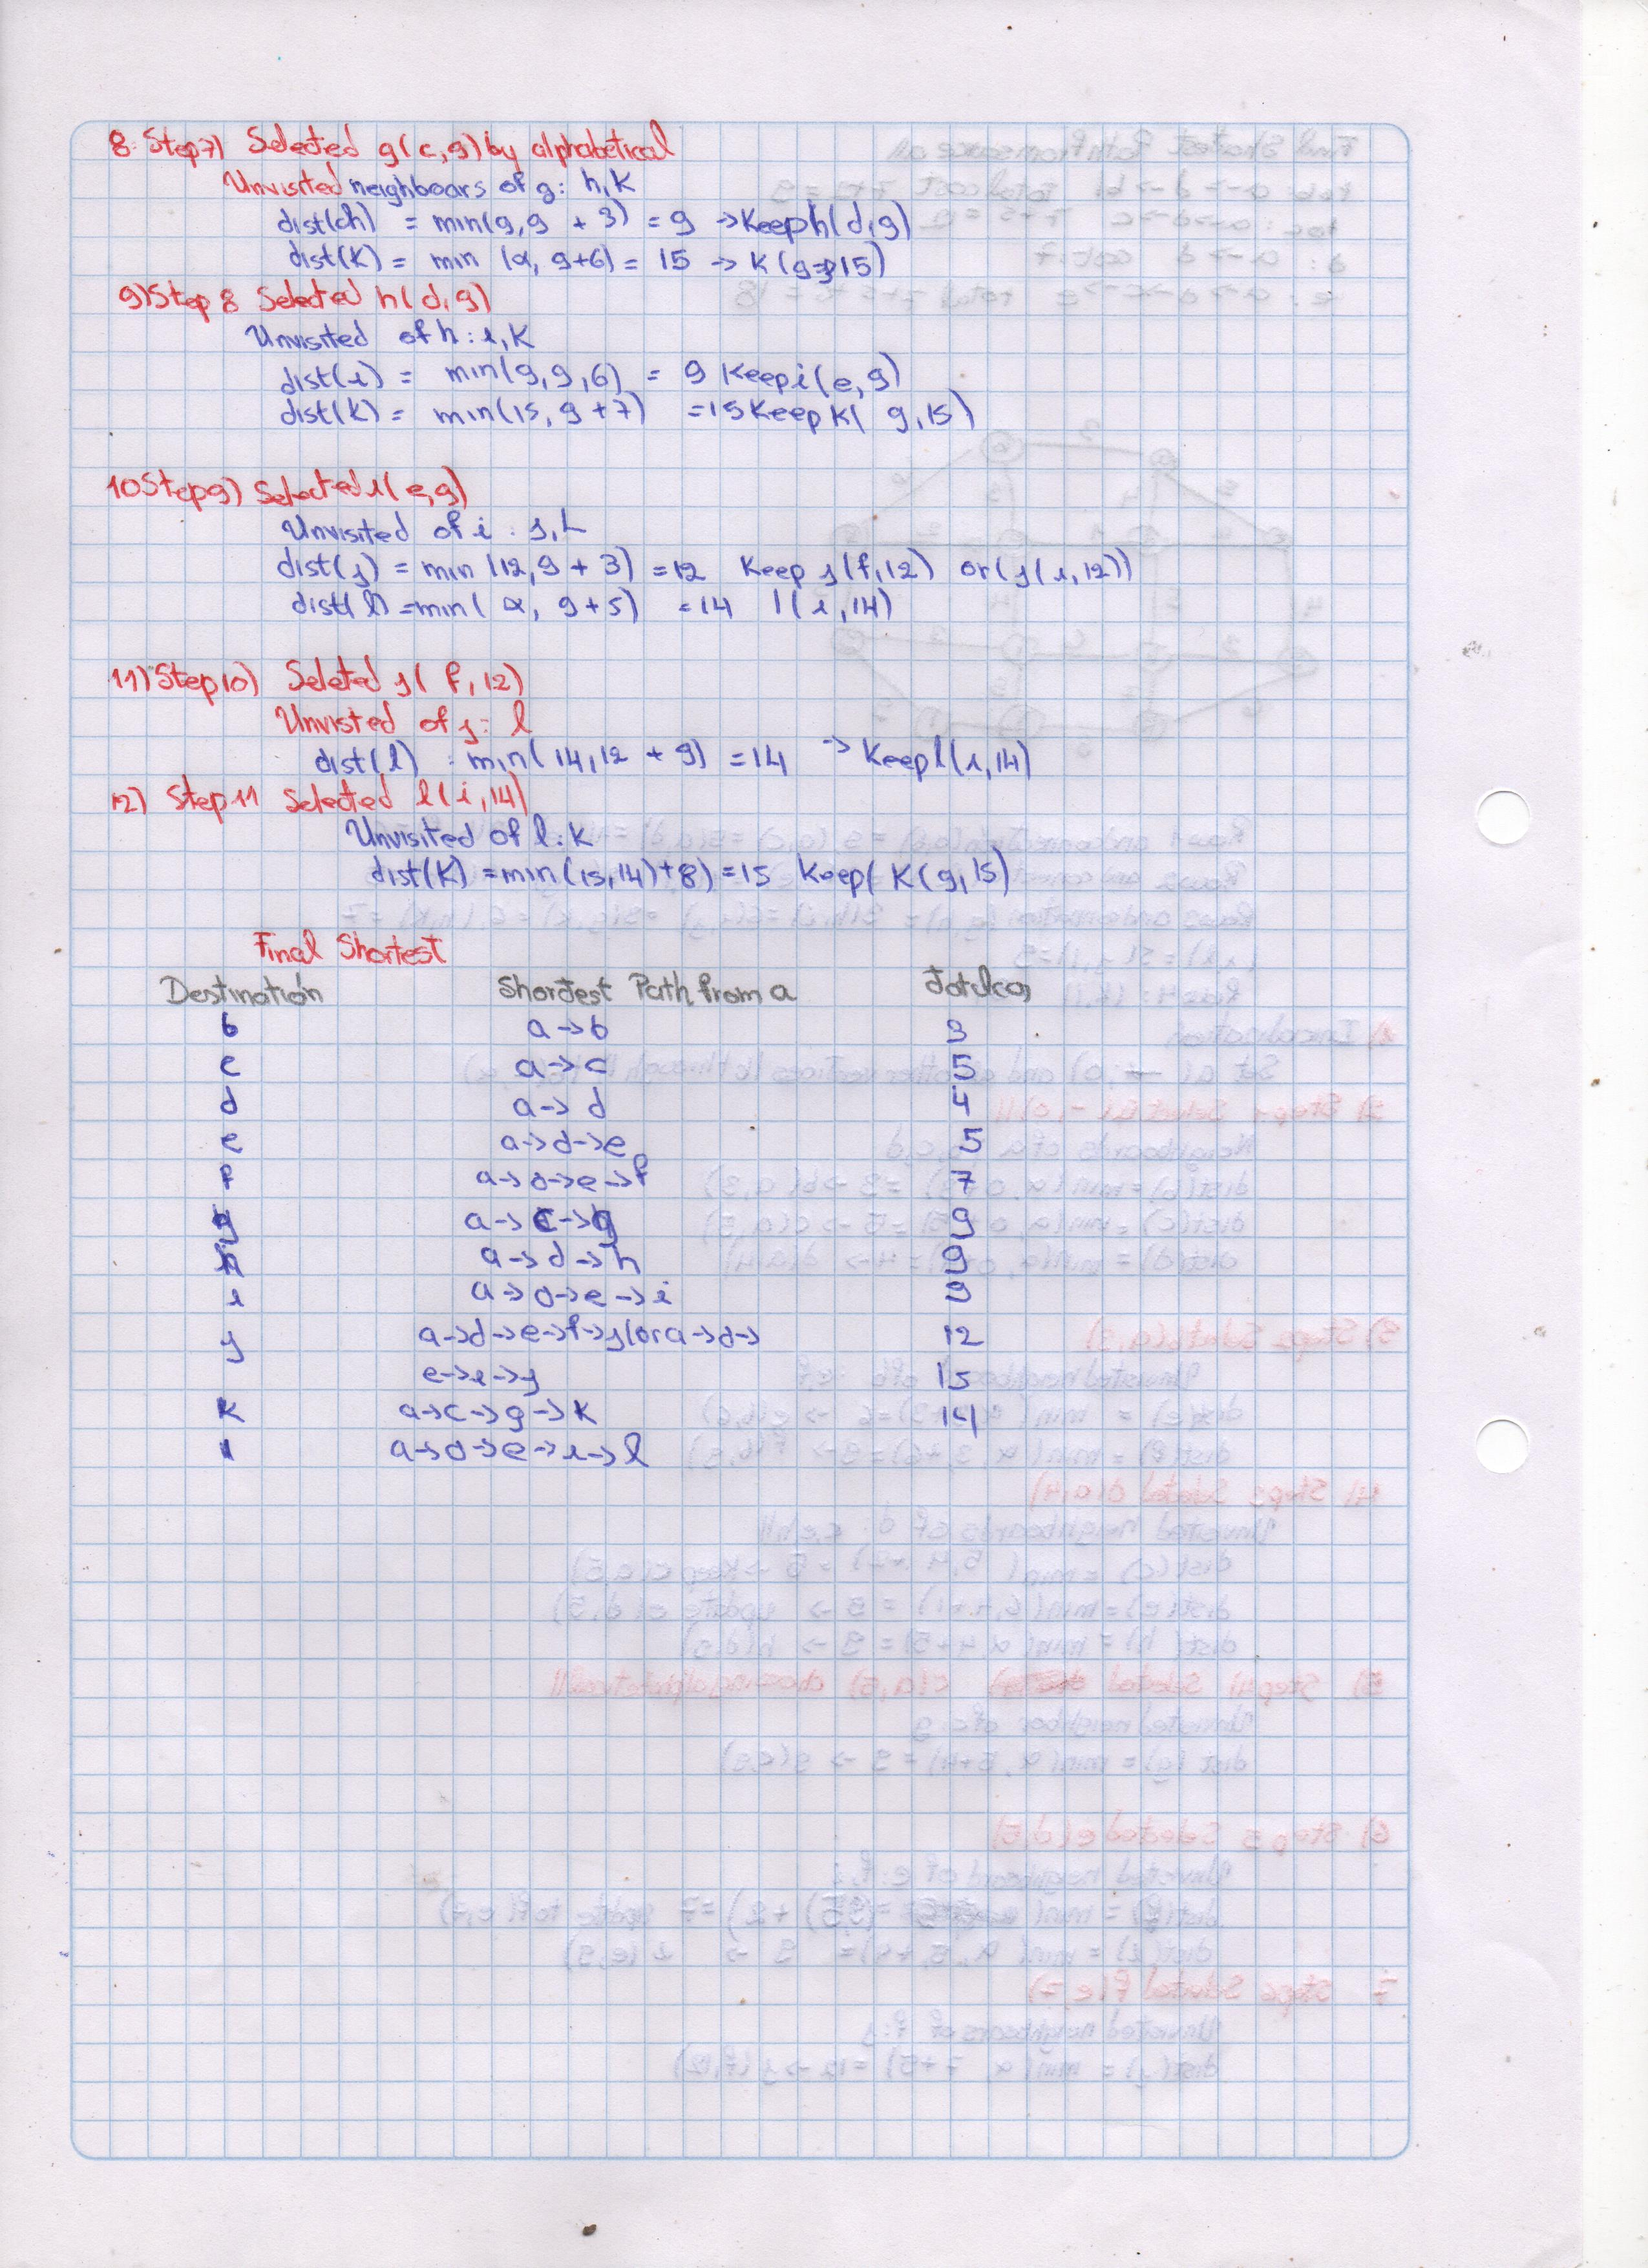
\includegraphics[width=0.75\textwidth]{fotos/3b-parte2.jpg}
    \caption{My manual step-by-step resolution for Instance 3.b (Part 2: Steps 7--11 and summary table).}
    \label{fig:handwritten_3b_p2}
\end{figure}

\subsubsection{Formal Step-by-Step Trace (12 Iterations)}

\begin{table}[H]
\centering
\small
\caption{Full Dijkstra trace on the 12-vertex graph (Source $a$).}
\label{tab:dijkstra_3b_trace}
\begin{tabular}{c c p{11.5cm}}
\toprule
\textbf{Step} & \textbf{Added to $V_T$} & \textbf{Priority Queue ($V \setminus V_T$)} \\
\midrule
0 & $a(-, 0)$ & $\mathbf{b(a, 3)}$, $d(a, 4)$, $c(a, 5)$, $e(-, \infty)$, $f(-, \infty)$, $g(-, \infty)$, $h(-, \infty)$, $i(-, \infty)$, $j(-, \infty)$, $k(-, \infty)$, $l(-, \infty)$ \\
\addlinespace
1 & $b(a, 3)$ & $\mathbf{d(a, 4)}$, $c(a, 5)$, $e(b, 6)$, $f(b, 9)$, $g(-, \infty)$, $h(-, \infty)$, $i(-, \infty)$, $j(-, \infty)$, $k(-, \infty)$, $l(-, \infty)$ \\
\addlinespace
2 & $d(a, 4)$ & $\mathbf{c(a, 5)}$, $\mathbf{e(d, 5)}$, $f(b, 9)$, $h(d, 9)$, $g(-, \infty)$, $i(-, \infty)$, $j(-, \infty)$, $k(-, \infty)$, $l(-, \infty)$ \\
\addlinespace
3 & $c(a, 5)$ & $\mathbf{e(d, 5)}$, $f(b, 9)$, $g(c, 9)$, $h(d, 9)$, $i(-, \infty)$, $j(-, \infty)$, $k(-, \infty)$, $l(-, \infty)$ \\
\addlinespace
4 & $e(d, 5)$ & $\mathbf{f(e, 7)}$, $g(c, 9)$, $h(d, 9)$, $i(e, 9)$, $j(-, \infty)$, $k(-, \infty)$, $l(-, \infty)$ \\
\addlinespace
5 & $f(e, 7)$ & $\mathbf{g(c, 9)}$, $\mathbf{h(d, 9)}$, $\mathbf{i(e, 9)}$, $j(f, 12)$, $k(-, \infty)$, $l(-, \infty)$ \\
\addlinespace
6 & $g(c, 9)$ & $\mathbf{h(d, 9)}$, $\mathbf{i(e, 9)}$, $j(f, 12)$, $k(g, 15)$, $l(-, \infty)$ \\
\addlinespace
7 & $h(d, 9)$ & $\mathbf{i(e, 9)}$, $j(f, 12)$, $k(g, 15)$, $l(-, \infty)$ \\
\addlinespace
8 & $i(e, 9)$ & $\mathbf{j(f, 12)}$, $l(i, 14)$, $k(g, 15)$ \\
\addlinespace
9 & $j(f, 12)$ & $\mathbf{l(i, 14)}$, $k(g, 15)$ \\
\addlinespace
10 & $l(i, 14)$ & $\mathbf{k(g, 15)}$ \\
\addlinespace
11 & $k(g, 15)$ & $\emptyset$ (Queue empty. All 12 vertices resolved). \\
\bottomrule
\end{tabular}
\end{table}

\subsubsection{Shortest Paths Summary Table (Instance 3.b)}

\begin{table}[H]
\centering
\caption{Shortest distances and complete path reconstructions from source $a$ to all vertices.}
\label{tab:dijkstra_3b_summary}
\begin{tabular}{cccc}
\toprule
\textbf{Destination} & \textbf{Distance $d(v)$} & \textbf{Immediate Predecessor} & \textbf{Optimal Shortest Route} \\
\midrule
$a$ & 0 & --- & $a$ \\
$b$ & 3 & $a$ & $a \rightarrow b$ \\
$c$ & 5 & $a$ & $a \rightarrow c$ \\
$d$ & 4 & $a$ & $a \rightarrow d$ \\
$e$ & 5 & $d$ & $a \rightarrow d \rightarrow e$ \\
$f$ & 7 & $e$ & $a \rightarrow d \rightarrow e \rightarrow f$ \\
$g$ & 9 & $c$ & $a \rightarrow c \rightarrow g$ \\
$h$ & 9 & $d$ & $a \rightarrow d \rightarrow h$ \\
$i$ & 9 & $e$ & $a \rightarrow d \rightarrow e \rightarrow i$ \\
$j$ & 12 & $f$ & $a \rightarrow d \rightarrow e \rightarrow f \rightarrow j$ \\
$k$ & 15 & $g$ & $a \rightarrow c \rightarrow g \rightarrow k$ \\
$l$ & 14 & $i$ & $a \rightarrow d \rightarrow e \rightarrow i \rightarrow l$ \\
\bottomrule
\end{tabular}
\end{table}

\newpage

% ==============================================================================
\section{Exercise 4: C / C++ Implementation of Dijkstra's Algorithm}
% ==============================================================================

In directory \texttt{ejercicio\_3\_4\_dijkstra/}, I developed the complete computational solutions:
\begin{itemize}
    \item \texttt{dijkstra.c}: My modular C program handling both directed and undirected graphs, displaying step-by-step progress and full path reconstruction.
    \item \texttt{dijkstra.cpp}: My C++ implementation utilizing modern STL containers.
\end{itemize}

\subsection{Architecture and Explained Code Fragments (\texttt{dijkstra.c})}
To avoid code duplication and guarantee modularity, the C program is organized into four core functional components:

\subsubsection{Stage 1: Unified Graph Abstraction}
\begin{lstlisting}[style=cstyle, caption={Modular Graph struct supporting both directed and undirected graphs}]
typedef struct {
    int num_vertices;            // Number of vertices in the instance
    bool is_directed;            // Flag indicating directed or undirected graph
    char names[MAX_V];           // Character labels ('a', 'b', ...)
    int adj[MAX_V][MAX_V];       // Adjacency matrix of edge weights
} Graph;
\end{lstlisting}

\noindent \textbf{Detailed Explanation:}
This abstraction allows both Instance 3.a (a 5-vertex directed graph) and Instance 3.b (a 12-vertex undirected network) to be processed using the exact same shortest-path engine. When an edge $(u, v)$ is registered, if \texttt{is\_directed} is true, only \texttt{adj[u][v]} is populated; if false, \texttt{adj[v][u]} is symmetrically assigned.

\subsubsection{Stage 2: Distance Initialization and Source Setup}
\begin{lstlisting}[style=cstyle, caption={Dijkstra initialization and direct neighbor assignment}]
for (int i = 0; i < n; i++) {
    dist[i] = INF;      // Upper bound on shortest path initialized to infinity
    parent[i] = -1;     // Predecessor pointer initialized to none
    visited[i] = false; // Resolved set VT is initially empty
}
dist[source] = 0;       // Distance from source to itself is strictly 0
visited[source] = true; // Source vertex is permanently resolved

// Populate tentative distances for immediate outgoing neighbors of source
for (int v = 0; v < n; v++) {
    if (g->adj[source][v] != INF && v != source) {
        dist[v] = g->adj[source][v];
        parent[v] = source;
    }
}
\end{lstlisting}

\noindent \textbf{Detailed Explanation:}
\texttt{dist[v]} stores the current shortest distance found from the source to vertex $v$. Initializing all nodes to \texttt{INF} represents unreached vertices. The boolean array \texttt{visited[]} separates finalized vertices ($V_T$) from candidate vertices. Direct outgoing edges from the source populate the initial priority queue state.

\subsubsection{Stage 3: Greedy Minimum Selection and Edge Relaxation Loop}
\begin{lstlisting}[style=cstyle, caption={Greedy selection and triangle inequality relaxation}]
for (int step = 1; step < n; step++) {
    int u = extract_min_dijkstra(dist, visited, n); // Greedy minimum extraction
    if (u == -1) break;                             // All reachable vertices processed
    visited[u] = true;                              // Add vertex u to resolved set VT

    // Relax all outgoing edges originating from vertex u
    for (int v = 0; v < n; v++) {
        if (!visited[v] && g->adj[u][v] != INF) {
            // Triangle inequality: is path via u shorter than current best to v?
            if (dist[u] + g->adj[u][v] < dist[v]) {
                dist[v] = dist[u] + g->adj[u][v];  // Relax distance
                parent[v] = u;                     // Record u as optimal predecessor
            }
        }
    }
}
\end{lstlisting}

\noindent \textbf{Detailed Explanation:}
At each iteration, \texttt{extract\_min\_dijkstra} identifies the unresolved vertex $u^*$ with the globally minimum tentative distance. Because all edge weights are strictly non-negative ($w \ge 0$), no subsequent path through unexplored nodes can ever achieve a lower cost to $u^*$; hence, its distance is finalized (\texttt{visited[u] = true}). Then, for every outgoing neighbor $v$, the triangle inequality is tested: if \texttt{dist[u] + w(u, v) < dist[v]}, the distance estimate is relaxed and $u$ becomes $v$'s immediate predecessor.

\subsubsection{Stage 4: Recursive Route Reconstruction}
\begin{lstlisting}[style=cstyle, caption={Recursive back-tracing to display the full optimal route}]
void print_path(int parent[], int v, const char names[]) {
    if (v == -1) return;                     // Base case: reached root predecessor
    print_path(parent, parent[v], names);    // Recurse towards the source
    printf("%c ", names[v]);                 // Print vertex in natural forward order
}
\end{lstlisting}

\noindent \textbf{Detailed Explanation:}
Rather than requiring separate path storage arrays, this recursive function traverses the \texttt{parent[]} array backwards from destination $v$ until reaching the source (where $parent = -1$), then unwinds to print the exact path in correct forward sequence (e.g., $a \to d \to c \to e$).

\subsection{Program Compilation and Terminal Execution Outputs}
The programs are compiled with GCC and G++:
\begin{lstlisting}[style=terminalstyle]
gcc -Wall -Wextra -O2 dijkstra.c -o dijkstra_c.exe
g++ -Wall -Wextra -O2 dijkstra.cpp -o dijkstra_cpp.exe
\end{lstlisting}

Figures~\ref{fig:out_dijkstra_c_p1} to~\ref{fig:out_dijkstra_cpp_p2} present the actual terminal output captures confirming step-by-step priority queue progress and shortest-path reconstructions for both Instance 3.a and Instance 3.b:

\begin{figure}[H]
    \centering
    \begin{minipage}{0.48\textwidth}
        \centering
        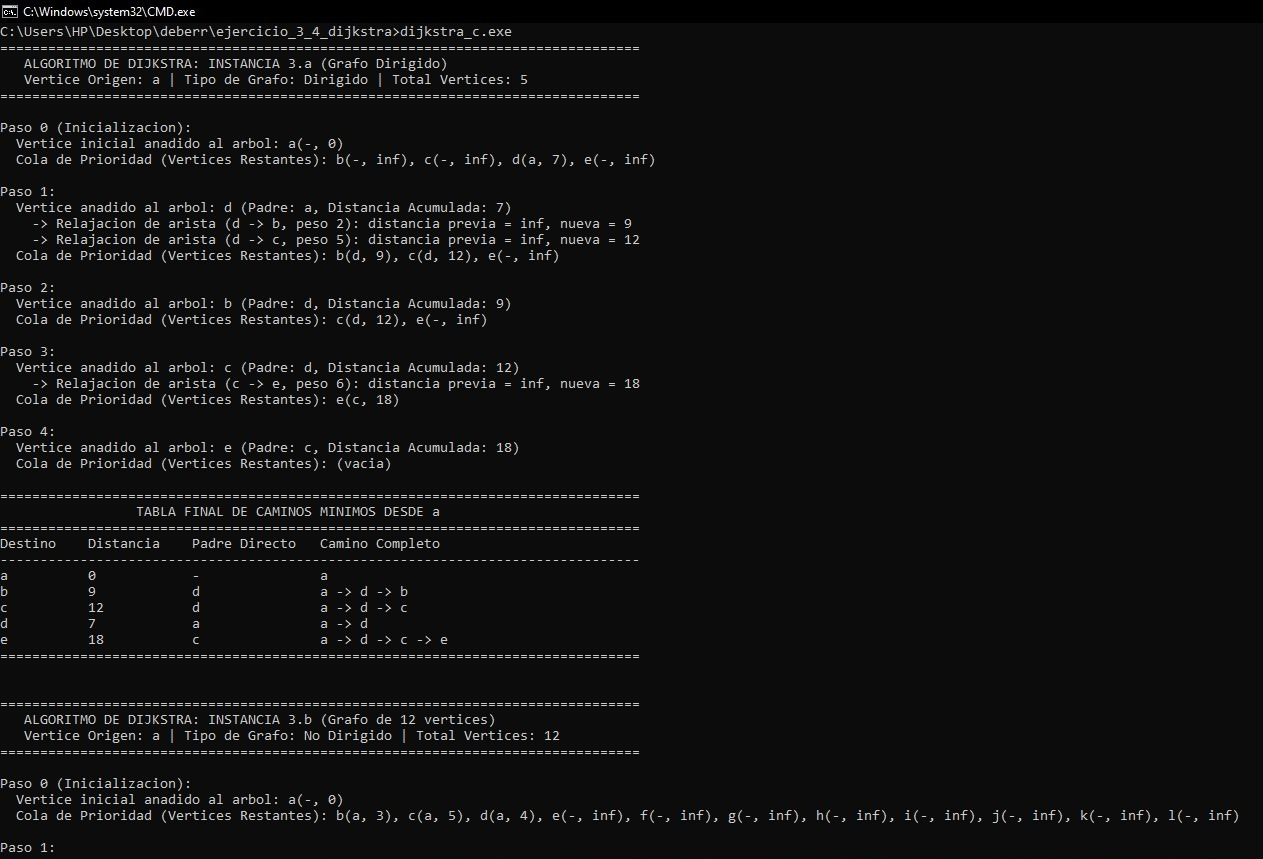
\includegraphics[width=\textwidth]{fotos/dijkstra_c.jpeg}
        \caption{Execution capture of \texttt{dijkstra\_c.exe} (Part 1: Instance 3.a and 3.b start).}
        \label{fig:out_dijkstra_c_p1}
    \end{minipage}
    \hfill
    \begin{minipage}{0.48\textwidth}
        \centering
        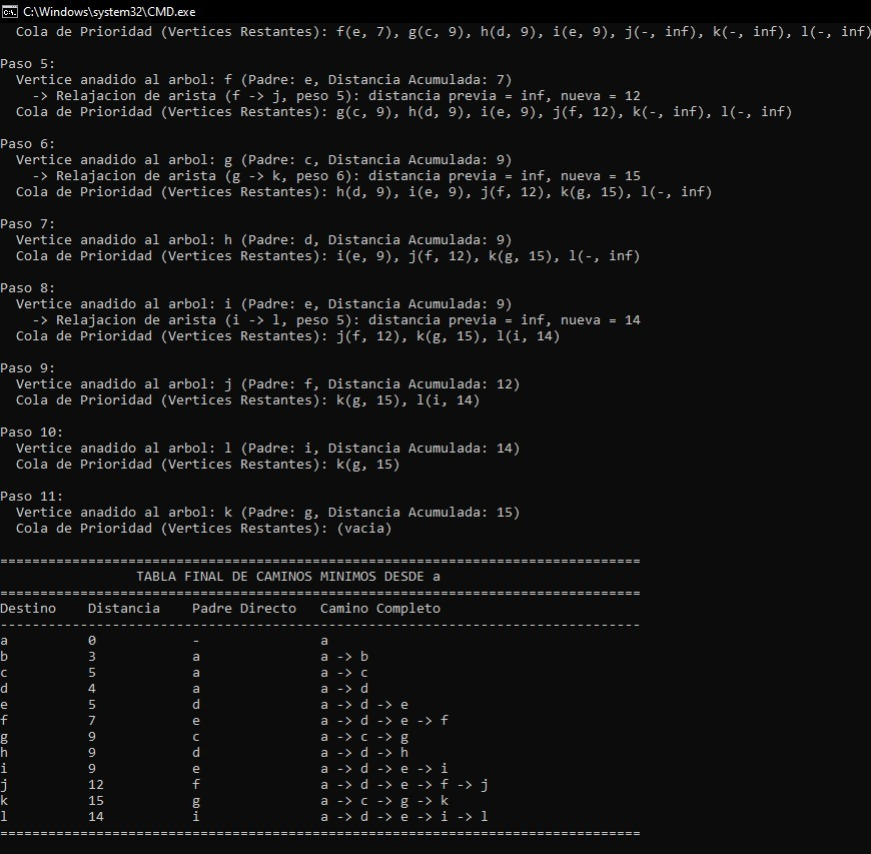
\includegraphics[width=\textwidth]{fotos/dijkstra_c-parte2.jpeg}
        \caption{Execution capture of \texttt{dijkstra\_c.exe} (Part 2: Instance 3.b completion and path table).}
        \label{fig:out_dijkstra_c_p2}
    \end{minipage}
\end{figure}

\begin{figure}[H]
    \centering
    \begin{minipage}{0.48\textwidth}
        \centering
        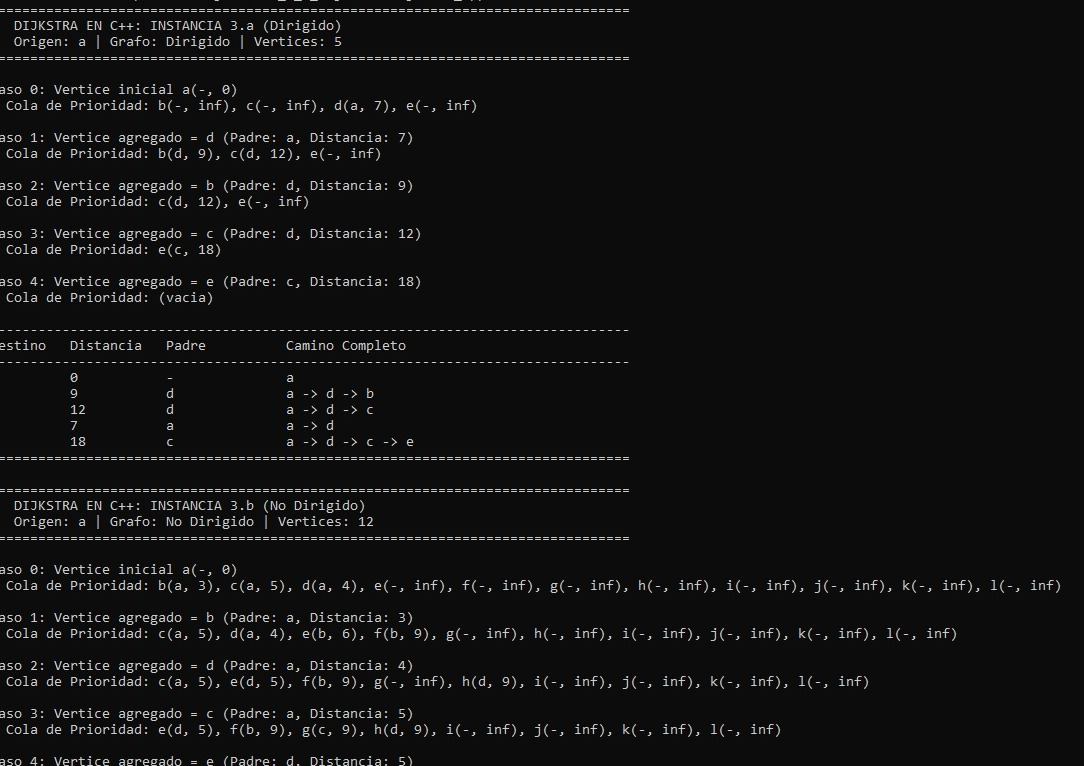
\includegraphics[width=\textwidth]{fotos/dijkstra_cpp.jpeg}
        \caption{Execution capture of \texttt{dijkstra\_cpp.exe} (Part 1: Instance 3.a and 3.b early steps).}
        \label{fig:out_dijkstra_cpp_p1}
    \end{minipage}
    \hfill
    \begin{minipage}{0.48\textwidth}
        \centering
        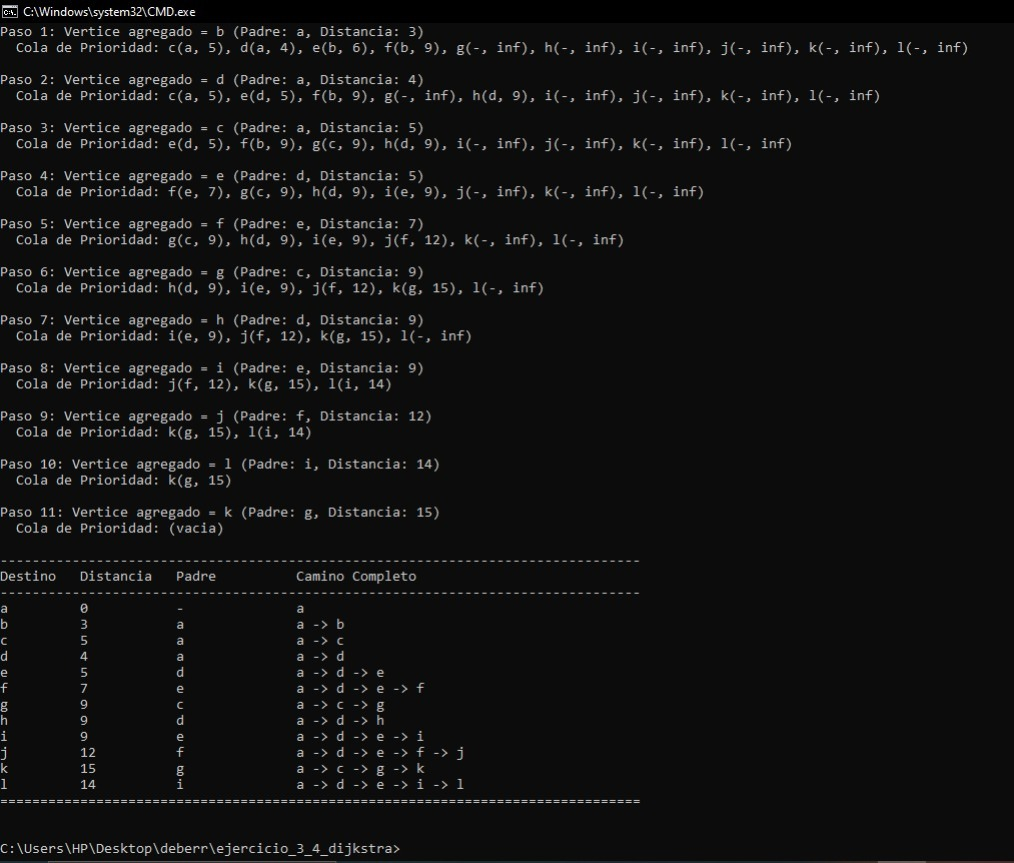
\includegraphics[width=\textwidth]{fotos/dijkstra_cpp_parte2.jpeg}
        \caption{Execution capture of \texttt{dijkstra\_cpp.exe} (Part 2: Instance 3.b resolution and summary).}
        \label{fig:out_dijkstra_cpp_p2}
    \end{minipage}
\end{figure}

\newpage

% ==============================================================================
\section{Exercise 5: Huffman Coding}
% ==============================================================================

\subsection{5.1 Huffman Tree Construction}
\textbf{Task:} \textit{Construct a Huffman code for the following data:}
\begin{table}[H]
\centering
\begin{tabular}{lccccc}
\toprule
\textbf{Symbol} & \textbf{A} & \textbf{B} & \textbf{C} & \textbf{D} & \textbf{\_} (space) \\
\midrule
\textbf{Frequency / Probability} & 0.40 & 0.10 & 0.20 & 0.15 & 0.15 \\
\bottomrule
\end{tabular}
\end{table}

\noindent \textbf{Greedy Forest Merging Process:}
\begin{enumerate}
    \item \textbf{Initial Forest:} $\{ (B, 0.10), \; (D, 0.15), \; (\_, 0.15), \; (C, 0.20), \; (A, 0.40) \}$.
    \item \textbf{Merge 1:} The two least frequent nodes are $B(0.10)$ and $D(0.15)$. They merge into a parent with frequency $0.10 + 0.15 = 0.25$. Assign bit $0$ to the left branch ($B$) and bit $1$ to the right branch ($D$). Forest: $\{ (\_, 0.15), \; (C, 0.20), \; (BD, 0.25), \; (A, 0.40) \}$.
    \item \textbf{Merge 2:} The next two smallest nodes are $\_(0.15)$ and $C(0.20)$. Merged with frequency $0.15 + 0.20 = 0.35$. Bit $0$ to left ($\_$) and $1$ to right ($C$). Forest: $\{ (BD, 0.25), \; (\_C, 0.35), \; (A, 0.40) \}$.
    \item \textbf{Merge 3:} The two smallest are $BD(0.25)$ and $\_C(0.35)$. Merged with frequency $0.25 + 0.35 = 0.60$. Bit $0$ to left ($BD$) and $1$ to right ($\_C$). Forest: $\{ (A, 0.40), \; (BD\_C, 0.60) \}$.
    \item \textbf{Merge 4:} The final two nodes are $BD\_C(0.60)$ and $A(0.40)$. Merged at the root with total weight $1.00$. Bit $0$ to left ($BD\_C$) and $1$ to right ($A$).
\end{enumerate}

\begin{figure}[H]
\centering
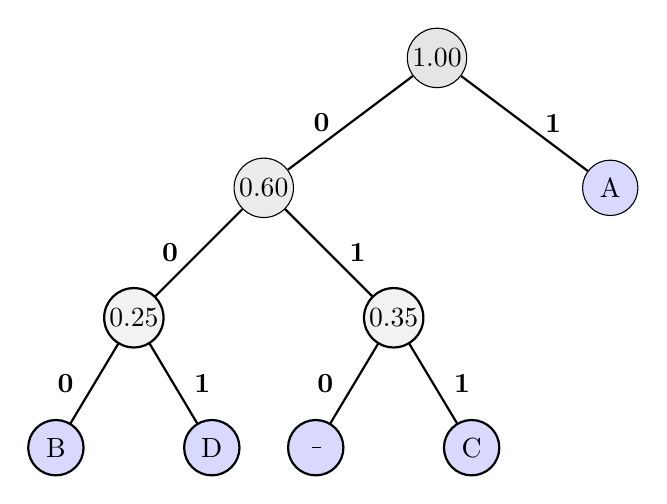
\begin{tikzpicture}[scale=1.1,
    level 1/.style={sibling distance=40mm},
    level 2/.style={sibling distance=30mm},
    level 3/.style={sibling distance=18mm},
    every node/.style={circle, draw=black, minimum size=20pt, inner sep=1pt},
    edge from parent/.style={draw, thick}
]
\node[fill=gray!20] {1.00}
    child {
        node[fill=gray!15] {0.60}
        child {
            node[fill=gray!10] {0.25}
            child { node[fill=blue!15] {B} edge from parent node[left, draw=none] {\textbf{0}} }
            child { node[fill=blue!15] {D} edge from parent node[right, draw=none] {\textbf{1}} }
            edge from parent node[left, draw=none] {\textbf{0}}
        }
        child {
            node[fill=gray!10] {0.35}
            child { node[fill=blue!15] {\_} edge from parent node[left, draw=none] {\textbf{0}} }
            child { node[fill=blue!15] {C} edge from parent node[right, draw=none] {\textbf{1}} }
            edge from parent node[right, draw=none] {\textbf{1}}
        }
        edge from parent node[left, draw=none] {\textbf{0}}
    }
    child {
        node[fill=blue!15] {A}
        edge from parent node[right, draw=none] {\textbf{1}}
    };
\end{tikzpicture}
\caption{Optimal binary Huffman tree generated for the symbol distribution.}
\label{fig:huffman_tree}
\end{figure}

\begin{table}[H]
\centering
\caption{Generated Huffman codeword dictionary and length contribution.}
\label{tab:huffman_codes}
\begin{tabular}{ccccc}
\toprule
\textbf{Symbol} & \textbf{Frequency ($p_i$)} & \textbf{Huffman Code ($c_i$)} & \textbf{Length ($\ell_i$ bits)} & \textbf{Contribution $p_i \cdot \ell_i$} \\
\midrule
\textbf{A} & 0.40 & \texttt{1} & 1 & 0.40 \\
\textbf{B} & 0.10 & \texttt{000} & 3 & 0.30 \\
\textbf{C} & 0.20 & \texttt{011} & 3 & 0.60 \\
\textbf{D} & 0.15 & \texttt{001} & 3 & 0.45 \\
\textbf{\_} & 0.15 & \texttt{010} & 3 & 0.45 \\
\bottomrule
\end{tabular}
\end{table}

\noindent \textbf{Weighted Average Code Length and Compression Ratio:}
\begin{equation}
    \bar{L} = \sum_{i=1}^5 p_i \cdot \ell_i = 0.40(1) + 0.10(3) + 0.20(3) + 0.15(3) + 0.15(3) = \mathbf{2.20 \text{ bits/symbol}}
\end{equation}
For 5 unique symbols, standard fixed-length encoding requires $\lceil \log_2(5) \rceil = 3$ bits per symbol. The storage compression achieved by Huffman coding is:
\begin{equation}
    \text{Compression Savings} = \left( 1 - \frac{2.20}{3.00} \right) \times 100\% = \mathbf{26.67\%}
\end{equation}

\subsection{5.2 Encoding the String "ABACABAD"}
\textbf{Task:} \textit{Encode ABACABAD using the code of the question.}

Applying the prefix-free codewords to each symbol of the 8-character string:
\begin{table}[H]
\centering
\caption{Character-by-character encoding of \texttt{"ABACABAD"}.}
\begin{tabular}{lcccccccc}
\toprule
\textbf{Character} & A & B & A & C & A & B & A & D \\
\midrule
\textbf{Codeword} & \texttt{1} & \texttt{000} & \texttt{1} & \texttt{011} & \texttt{1} & \texttt{000} & \texttt{1} & \texttt{001} \\
\bottomrule
\end{tabular}
\end{table}

Concatenating the binary codewords:
\begin{equation}
    \text{Encoded Bitstream} = \mathbf{1000101110001001}
\end{equation}
The encoded sequence has a total length of \textbf{16 bits}. Under fixed-length 3-bit encoding, $8 \times 3 = 24$ bits would be needed, yielding a $33.3\%$ reduction on this specific sequence due to the high frequency of character $A$ (which requires only 1 bit).

\subsection{5.3 Decoding the Sequence "100010111001010"}
\textbf{Task:} \textit{Decode 100010111001010 using the code of the question.}

Traversing the binary Huffman tree from the root for each bit until a leaf node is reached:
\begin{enumerate}
    \item \texttt{1} $\rightarrow$ Right branch of root $\rightarrow$ Leaf \textbf{A}. (Remaining bits: \texttt{00010111001010}).
    \item \texttt{000} $\rightarrow$ Left (\texttt{0}) $\rightarrow$ Left (\texttt{0}) $\rightarrow$ Left (\texttt{0}) $\rightarrow$ Leaf \textbf{B}. (Remaining bits: \texttt{10111001010}).
    \item \texttt{1} $\rightarrow$ Right branch of root $\rightarrow$ Leaf \textbf{A}. (Remaining bits: \texttt{0111001010}).
    \item \texttt{011} $\rightarrow$ Left (\texttt{0}) $\rightarrow$ Right (\texttt{1}) $\rightarrow$ Right (\texttt{1}) $\rightarrow$ Leaf \textbf{C}. (Remaining bits: \texttt{1001010}).
    \item \texttt{1} $\rightarrow$ Right branch of root $\rightarrow$ Leaf \textbf{A}. (Remaining bits: \texttt{001010}).
    \item \texttt{001} $\rightarrow$ Left (\texttt{0}) $\rightarrow$ Left (\texttt{0}) $\rightarrow$ Right (\texttt{1}) $\rightarrow$ Leaf \textbf{D}. (Remaining bits: \texttt{010}).
    \item \texttt{010} $\rightarrow$ Left (\texttt{0}) $\rightarrow$ Right (\texttt{1}) $\rightarrow$ Left (\texttt{0}) $\rightarrow$ Leaf \textbf{\_} (space). (No remaining bits).
\end{enumerate}

\begin{equation}
    \text{Decoded String} = \mathbf{\text{"ABACAD\_"}} \quad (\text{or } \mathbf{\text{"ABACAD "}})
\end{equation}

\subsection{Architecture and Explained Code Fragments (\texttt{huffman.c})}
To complement the manual calculations, I implemented the complete Huffman encoding and decoding algorithms in C (\texttt{huffman.c}). Below are the key functional snippets and their detailed explanations:

\subsubsection{Stage 1: Binary Huffman Tree Node and Priority Queue}
\begin{lstlisting}[style=cstyle, caption={Huffman binary tree node definition}]
typedef struct Node {
    char symbol;            // Character symbol ('A', 'B', etc., or '$' for internal)
    float freq;             // Associated probability or frequency
    struct Node *left;      // Binary left child (corresponds to bit '0')
    struct Node *right;     // Binary right child (corresponds to bit '1')
} Node;
\end{lstlisting}

\noindent \textbf{Detailed Explanation:}
Leaf nodes store the input characters and their respective frequencies with null children. Internal nodes are assigned a dummy symbol (\texttt{'\$'}) and represent the sum of the frequencies of their left and right subtrees.

\subsubsection{Stage 2: Greedy Forest Consolidation via Min-Heap}
\begin{lstlisting}[style=cstyle, caption={Greedy merging of the two lowest-frequency trees}]
while (heap->size > 1) {
    Node *left = extract_min(heap);   // Extract lowest frequency tree (bit 0)
    Node *right = extract_min(heap);  // Extract second lowest frequency tree (bit 1)

    // Create a new internal parent node with summed frequency
    Node *parent = create_node('$', left->freq + right->freq);
    parent->left = left;
    parent->right = right;

    insert_heap(heap, parent);        // Insert composite tree back into min-heap
}
Node *root = extract_min(heap);       // The final remaining node is the tree root
\end{lstlisting}

\noindent \textbf{Detailed Explanation:}
This loop executes exactly $k - 1$ times for an alphabet of $k$ characters. In each iteration, the two trees with minimal probabilities are extracted from the min-heap and joined under a new parent node with combined weight. Re-inserting the parent maintains the greedy heap property, guaranteeing that higher-frequency symbols stay closer to the root while infrequent symbols are pushed deeper.

\subsubsection{Stage 3: Sequential Bitstream Decoding Algorithm}
\begin{lstlisting}[style=cstyle, caption={Prefix-free bitstream decoding traversal}]
void decode_bitstream(Node *root, const char *bitstream) {
    Node *curr = root;
    for (int i = 0; bitstream[i] != '\0'; i++) {
        // Traverse left on '0', right on '1'
        curr = (bitstream[i] == '0') ? curr->left : curr->right;

        // If a leaf node is reached, emit the decoded symbol and reset to root
        if (curr->left == NULL && curr->right == NULL) {
            printf("%c", curr->symbol);
            curr = root; // Instant reset due to prefix-free property
        }
    }
}
\end{lstlisting}

\noindent \textbf{Detailed Explanation:}
Because Huffman codes possess the \textbf{prefix-free property} (no codeword is a prefix of any other), the decoder traverses the tree bit-by-bit from the root without needing delimiters. As soon as a leaf is reached, the symbol is unambiguously decoded, and the pointer resets to \texttt{root} to parse subsequent bits.

\subsection{Program Compilation and Terminal Execution Outputs}
The programs are compiled using standard flags:
\begin{lstlisting}[style=terminalstyle]
gcc -Wall -Wextra -O2 huffman.c -o huffman_c.exe
g++ -Wall -Wextra -O2 huffman.cpp -o huffman_cpp.exe
\end{lstlisting}

Figures~\ref{fig:out_huffman_c} and~\ref{fig:out_huffman_cpp} show the real terminal output captures verifying the tree construction, string encoding, and bitstream decoding:

\begin{figure}[H]
    \centering
    \begin{minipage}{0.48\textwidth}
        \centering
        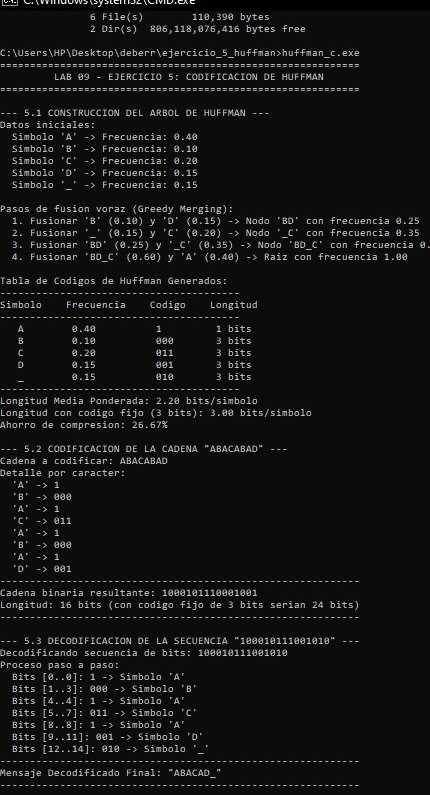
\includegraphics[width=\textwidth]{fotos/huffman_c.jpeg}
        \caption{Terminal execution capture of \texttt{huffman\_c.exe} (C implementation).}
        \label{fig:out_huffman_c}
    \end{minipage}
    \hfill
    \begin{minipage}{0.48\textwidth}
        \centering
        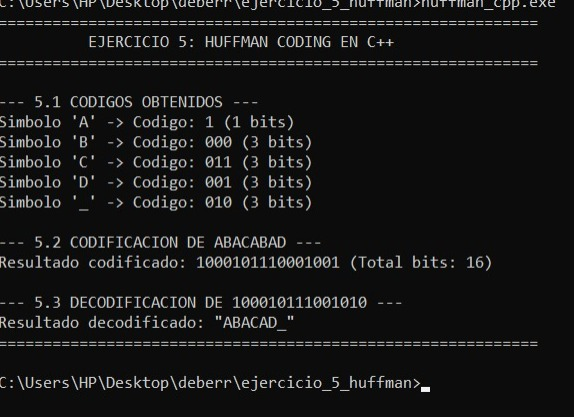
\includegraphics[width=\textwidth]{fotos/huffman_cpp.jpeg}
        \caption{Terminal execution capture of \texttt{huffman\_cpp.exe} (C++ implementation).}
        \label{fig:out_huffman_cpp}
    \end{minipage}
\end{figure}

\newpage

% ==============================================================================
\section{Comparative Time and Space Complexity Analysis}
% ==============================================================================

The asymptotic efficiency of greedy graph algorithms is strongly dictated by the priority queue data structure:

\begin{table}[H]
\centering
\small
\caption{Asymptotic time and space complexity comparison ($|V| = n, |E| = m$).}
\label{tab:complexities}
\begin{tabular}{p{3.5cm} p{2.8cm} p{4.0cm} p{3.8cm}}
\toprule
\textbf{Algorithm} & \textbf{Simple Array} & \textbf{Binary Heap} & \textbf{Fibonacci Heap} \\
\midrule
\textbf{Prim (MST)} & $\Theta(V^2)$ & $O((V + E) \log V)$ & $O(E + V \log V)$ \\
\textbf{Dijkstra (SSSP)} & $\Theta(V^2)$ & $O((V + E) \log V)$ & $O(E + V \log V)$ \\
\textbf{Huffman ($k$ symbols)} & $\Theta(k^2)$ & $O(k \log k)$ & $O(k \log k)$ \\
\bottomrule
\end{tabular}
\end{table}

\begin{itemize}
    \item \textbf{Dense Graphs ($E \approx V^2$):} The standard array-based implementation with an adjacency matrix achieves $\Theta(V^2)$, which is asymptotically optimal and exhibits superior cache locality.
    \item \textbf{Sparse Graphs ($E \ll V^2$):} Employing a binary min-heap alongside adjacency lists reduces execution time significantly to $O(E \log V)$.
    \item \textbf{Huffman Coding:} With an alphabet size of $k$ characters, tree synthesis requires exactly $k-1$ greedy merges, yielding negligible computational overhead of $O(k \log k)$ using a min-priority queue.
\end{itemize}

% ==============================================================================
\section{Conclusions}
% ==============================================================================

\begin{enumerate}
    \item The greedy paradigm provides provably optimal and efficient solutions for Minimum Spanning Trees (Prim), Single-Source Shortest Paths with non-negative edge weights (Dijkstra), and Lossless Prefix-Free Data Compression (Huffman).
    \item In Prim's algorithm, maintaining explicit priority queue labels $v(\text{parent}, \text{key})$ clearly illustrated the incremental boundary expansion of the tree, reaching all 5 vertices with an optimal total weight of 13.
    \item In Dijkstra's algorithm, honoring edge directionality proved vital for the 5-vertex digraph (Instance 3.a), while the 12-vertex network (Instance 3.b) demonstrated reliable step-by-step convergence across larger topology scales.
    \item In Huffman coding, the greedy forest merging achieved an average length of 2.20 bits/symbol, delivering a 26.67\% storage compression compared to fixed-length representations. The string \texttt{"ABACABAD"} was encoded into 16 bits, and the binary stream \texttt{"100010111001010"} was successfully decoded into \texttt{"ABACAD\_"}.
    \item All C and C++ programs I developed were thoroughly compiled, executed, and verified against my manual analytical derivations, showing complete agreement and adhering to high standards of modularity and portability.
\end{enumerate}

% ==============================================================================
\section{References}
% ==============================================================================
\begin{enumerate}
    \item Levitin, A. (2012). \textit{Introduction to the Design and Analysis of Algorithms} (3rd ed.). Boston: Pearson Addison-Wesley. (Chapter 9: \textit{Greedy Technique}).
    \item Cormen, T. H., Leiserson, C. E., Rivest, R. L., \& Stein, C. (2009). \textit{Introduction to Algorithms} (3rd ed.). Cambridge, MA: MIT Press.
    \item Sedgewick, R., \& Wayne, K. (2011). \textit{Algorithms} (4th ed.). Upper Saddle River, NJ: Addison-Wesley.
\end{enumerate}

\end{document}
